\documentclass[12pt]{report}
\usepackage[fontsize=13pt]{scrextend}
\usepackage[utf8]{vietnam}
\usepackage[utf8]{inputenc}
\usepackage[vietnamese]{babel}
\usepackage{titlesec}
\usepackage{titletoc}
\usepackage{listings}
\usepackage[bookmarks=true]{hyperref}
\usepackage[left=3cm,right=2cm,top=2.5cm,bottom=3cm]{geometry}
\usepackage{graphicx}
\usepackage{hyperref}
\usepackage{tikz}
\usepackage{varwidth}
\usepackage{float}
\usepackage{listings}
\usepackage{color}
\usepackage{multirow}
\usepackage{booktabs}
\usepackage[ruled,vlined]{algorithm2e}
\usepackage{chngcntr}
\usepackage{nameref}

%\usepackage[font=bf]{caption}
%\counterwithin{figure}{chapter}

\renewcommand\labelitemi{--}

\setlength{\parskip}{6pt}
\setcounter{secnumdepth}{4}
\usetikzlibrary{calc}
\setlength{\parindent}{10mm}
\renewcommand{\baselinestretch}{1.3}
\graphicspath{{images/}}

%%% The following lines add Chapter or Appendix in front of the number
\titlecontents{chapter}%
[0pt]%
{\vspace{1ex}}%
{\bfseries Chương \thecontentslabel\quad}%
{\bfseries}%
{\bfseries\hfill\contentspage}
%%% Initially, for the main part of the document, set the label to "Chapter"
\let\chapappname\chaptername

\definecolor{dkgreen}{rgb}{0,0.6,0}
\definecolor{gray}{rgb}{0.5,0.5,0.5}
\definecolor{mauve}{rgb}{0.58,0,0.82}

% setup code area as listings
\lstset{frame=tb,
  language=Python,
  aboveskip=3mm,
  belowskip=3mm,
  showstringspaces=false,
  columns=flexible,
  basicstyle={\small\ttfamily},
  numbers=left,
  numberstyle=\tiny\color{gray},
  keywordstyle=\color{blue},
  commentstyle=\color{dkgreen},
  stringstyle=\color{mauve},
  breaklines=true,
  breakatwhitespace=true,
  tabsize=3
}

\renewcommand{\lstlistingname}{Mã nguồn}

\newenvironment{thuattoan}[1][h]
  {\renewcommand{\algorithmcfname}{Thuật toán}
   \begin{algorithm}[#1]
  }{\end{algorithm}}

% hyper setup
\hypersetup{
	bookmarks=true,
	pdftitle={MÔ HÌNH TÌM KIẾM ĐOẠN NỘI DUNG TƯƠNG
	ĐỒNG GIỮA CÁC VĂN BẢN KHÔNG CÙNG NGÔN
	NGỮ},
	pdfauthor={Trần Minh Chiến}, % author
	pdfsubject={TeX and LaTeX},
	pdfkeywords={TeX, LaTeX, graphics, images}, % list of keywords
	colorlinks=false,       % false: boxed links; true: colored links
	linkcolor=black,       % color of internal links
	citecolor=black,       % color of links to bibliography
	filecolor=black,        % color of file links
	urlcolor=black,        % color of external links
	linktoc=page            % only page is linked
}

\begin{document}
\begin{titlepage}
	\center
	\begin{tikzpicture}[overlay,remember picture]
		\draw [line width=3pt,rounded corners=0pt,]
		($ (current page.north west) + (25mm,-25mm) $)
		rectangle
		($ (current page.south east) + (-15mm,25mm) $);
		\draw [line width=1pt,rounded corners=0pt]
		($ (current page.north west) + (26.5mm,-26.5mm) $)
		rectangle
		($ (current page.south east) + (-16.5mm,26.5mm) $);
	\end{tikzpicture}
	
	{\large \bfseries ĐẠI HỌC QUỐC GIA HÀ NỘI\\ TRƯỜNG ĐẠI HỌC CÔNG NGHỆ}\\[1cm]
	
\includegraphics[width=0.2\linewidth]{uet}\\[1cm]
	{\Large  \bfseries Trần Minh Chiến}\\[1.5cm]
	{ \Large \bfseries MÔ HÌNH TÌM KIẾM ĐOẠN NỘI DUNG TƯƠNG
	ĐỒNG GIỮA CÁC VĂN BẢN KHÔNG CÙNG NGÔN
	NGỮ}\\[0.5cm]
	\hfill\\[1.5cm]
	{\large \bfseries KHÓA LUẬN TỐT NGHIỆP ĐẠI HỌC HỆ CHÍNH QUY}\\	
	{\large \bfseries Ngành: Công nghệ thông tin}	
	\hfill\\[3.5cm]	
	{\large \bfseries HÀ NỘI - 2019}\\	
	\vfill
\end{titlepage}
	
%-----SECONDARY TITLE PAGE-----%	
\begin{titlepage}
	\center
	\begin{tikzpicture}[overlay,remember picture]
		\draw [line width=3pt,rounded corners=0pt,]
		($ (current page.north west) + (25mm,-25mm) $)
		rectangle
		($ (current page.south east) + (-15mm,25mm) $);
		\draw [line width=1pt,rounded corners=0pt]
		($ (current page.north west) + (26.5mm,-26.5mm) $)
		rectangle
		($ (current page.south east) + (-16.5mm,26.5mm) $);
	\end{tikzpicture}
	
	{\large \bfseries ĐẠI HỌC QUỐC GIA HÀ NỘI\\ TRƯỜNG ĐẠI HỌC CÔNG NGHỆ}\\[2cm]
	{\Large  \bfseries Trần Minh Chiến}\\[2cm]		
	{ \Large \bfseries MÔ HÌNH TÌM KIẾM ĐOẠN NỘI DUNG TƯƠNG
	ĐỒNG GIỮA CÁC VĂN BẢN KHÔNG CÙNG NGÔN
	NGỮ}\\[0.5cm]
	\hfill\\[1.5cm]
	{\large \bfseries KHÓA LUẬN TỐT NGHIỆP ĐẠI HỌC HỆ CHÍNH QUY}\\	
	{\large \bfseries Ngành: Công nghệ thông tin}
	\hfill\\[1cm]
	\begin{flushleft}
		{\large \bfseries Cán bộ hướng dẫn: PGS.TS. Nguyễn Việt Hà}\\	
	\end{flushleft}
	\hfill\\[2cm]
	\begin{flushleft}
		{\large \bfseries Cán bộ đồng hướng dẫn: TS. Nguyễn Thị Ngọc Diệp}\\	
	\end{flushleft}
	\hfill\\[2cm]		
	{\large \bfseries HÀ NỘI - 2019}\\		
	\vfill		
\end{titlepage}

%-----TERTIARY TITLE PAGE-----%	
\begin{titlepage}
	\center
	\begin{tikzpicture}[overlay,remember picture]
	\draw [line width=3pt,rounded corners=0pt,]
	($ (current page.north west) + (25mm,-25mm) $)
	rectangle
	($ (current page.south east) + (-15mm,25mm) $);
	\draw [line width=1pt,rounded corners=0pt]
	($ (current page.north west) + (26.5mm,-26.5mm) $)
	rectangle
	($ (current page.south east) + (-16.5mm,26.5mm) $);
	\end{tikzpicture}
	
	{\large \bfseries VIETNAM NATIONAL UNIVERSITY, HA NOI\\ UNIVERSITY OF ENGINEERING AND TECHNOLOGY}\\[2cm]
	
	{\Large  \bfseries Tran Minh Chien}\\[2cm]		
	{ \LARGE \bfseries A CROSS-LANGUAGE  PRARGRAPH RETRIEVAL MODEL BASED ON DOCUMENT SIMILARITY}\\[0.2cm]
	\hfill\\[1.5cm]
	{\large \bfseries BACHELOR'S THESIS}\\	
	{\large \bfseries Major: Information Technology}
	\hfill\\[1cm]
	\begin{flushleft}
		{\large \bfseries Supervisor: Assoc.Prof. Nguyen Viet Ha}\\	
	\end{flushleft}
	\hfill\\[2cm]
	\begin{flushleft}
		{\large \bfseries Co-Supervisor: Dr. Nguyen Thi Ngoc Diep}\\	
	\end{flushleft}
	\hfill\\[2cm]			
	{\large \bfseries HANOI - 2019}\\		
	\vfill		
\end{titlepage}

%-----THANKS-----%
\newpage
\pagenumbering{roman}
\begin{center}
	\textbf{\large LỜI CẢM ƠN}
\end{center}
Đầu tiên, tôi muốn gửi lời cảm ơn chân thành đến PGS.TS Nguyễn Việt Hà, TS. Nguyễn Thị Ngọc Diệp, và ThS. Nguyễn Ngọc Khương - những người đã trực tiếp hướng dẫn chỉ bảo để tôi có thể hoàn thiện khóa luận này.

Tôi xin được cảm ơn các thầy, cô tại trường đại học Công Nghệ - Đại học Quốc gia Hà Nội, tập thể lớp K60 CLC đã đồng hành cùng với tôi trong suốt bốn năm qua, đã chỉ bảo, giúp đỡ tôi những những lúc khó khăn cũng như đã tạo ra môi trường lý tưởng cho tôi được phát triển.

Tôi cũng xin gửi lời cảm ơn đến tập thể thành viên SkyLab, những người đã đồng hành cùng với tôi trong suốt quá trình nghiên cứu cũng như xây dựng khóa luận này.

Cuối cùng tôi xin dành lời cảm ơn đến gia đình, những người là động lực để tôi cố gắng rèn luyện, hoàn thiện mình hơn và tới bạn Dương Minh Thu, người đã động viên cũng như giúp đỡ tôi vượt qua những khó khăn để hoàn thiện khóa luận này.

Tôi xin chân thành cảm ơn !

	
%-----ABSTRACT-----%
\newpage
\begin{center}
	\textbf{\large TÓM TẮT}
\end{center}
Khóa luận này trình bày một mô hình tìm kiếm đoạn nội dung tương đồng giữa các văn bản không cùng ngôn ngữ trong đó đầu vào là một văn bản của ngôn ngữ tiếng Việt  và đầu ra là những đoạn văn bản có nội dung tương đồng của ngôn ngữ tiếng Anh.

Mô hình tìm kiếm đoạn nội dung tương đồng này dựa trên các thuật toán xử lý ngôn ngữ tự nhiên, công cụ dịch thuật và các phương pháp tính toán độ tương tự dựa trên nội dung để tìm kiếm và xếp hạng các đoạn văn bản trong một tập dữ liệu tiếng Anh  đã được thu thập từ nhiều nguồn. 

Mô hình được xây dựng dựa trên ba phần chính bao gồm:
\begin{itemize}
	\item Mô-đun thu thập dữ liệu: tự động thu thập dữ liệu văn bản tiếng Anh từ nhiều nguồn làm cơ sở dữ liệu truy xuất.
	\item Mô-đun xử lý và truy xuất văn bản (mô-đun chính): thực hiện tách đoạn văn bản, vector hoá đoạn văn bản, ánh xạ từ khoá, và tính toán độ tương đồng giữa các văn bản.
	\item Mô-đun giao diện người dùng: cho phép người dùng nhập một đoạn văn bản tiếng Việt và trả lại một dãy các kết quả đã được xếp hạng
\end{itemize}

Khoá luận đồng thời chỉ ra khả năng áp dụng của mô hình cho bài toán tìm kiếm cũng như bài toán xác định đạo văn giữa các văn bản không cùng ngôn ngữ. 

Với phương pháp ma trận véc-tơ được đề xuất đã cho kết quả khả quan với độ tìm kiếm chính xác 66\% với số lượng kết quả trả về là một đoạn tương đồng gần nhất và 78\% khi số lượng kết quả trả về là ba. 


\noindent \textit{\textbf{Từ khóa:} Nội dung tương đồng, đa ngôn ngữ, nhận biết đạo văn
}

%-----ABSTRACT (ENGLISH)-----%
\newpage
\begin{center}
	\textbf{\large ABSTRACT}
\end{center}

This thesis proposes a model for finding similar paragraphs cross-language in which the input is a text written in Vietnamese and the output is the English text with similar content.
The model based on natural language processing algorithms, translation tools and statistical methods for searching in data sets which has been collected from various sources.

The model is built on three main parts:
\begin{itemize}
	\item Data collecting module: Automatically collect data about English text from multiple sources to build a retrieval database.
	\item Text processing and retrieval module (main module): Performs paragraph splitting, vectorize text, do mapping keywords, and calculate similarities between documents.
	\item User interface module: Allow users input a Vietnamese paragraph and return the ranked results.
\end{itemize}
The thesis simultaneously depict the applicable ability of the model in searching data as well as identifying the plagiarism between cross language texts.

With the Matrix method, the result is quite precise with searching match rate is 66\% with the return rate is one paragraph having similar content, and 78\% with the return rate is 3 paragraphs which are similar in content.

\noindent \textit{\textbf{Keywords:} content-based similarity, cross-language paragraph, retrieval plagiarism detection}

%-----UNDERTAKING-----%
\newpage
\begin{center}
	\textbf{\large LỜI CAM ĐOAN}
\end{center}
Tôi xin cam đoan toàn bộ khóa luận về mô hình tìm kiếm đoạn nội dung tương đồng giữa các văn bản không cùng ngôn ngữ, giao diện ứng dụng và phần mềm hệ thống là do tôi thực hiện dưới sự hướng dẫn của PGS. TS. Nguyễn Việt Hà và TS. Nguyễn Thị Ngọc Diệp

Những mô hình, phương pháp nghiên cứu liên quan đến khóa luận này đều đã được tôi trích dẫn và ghi chú rõ ràng trong danh sách những tài liệu tham khảo.

\begin{flushright}
	\begin{varwidth}{\linewidth}\centering
		Hà Nội, ngày 26 tháng 04 năm 2019\\
		Sinh viên\\[2cm]
		Trần Minh Chiến
	\end{varwidth}
\end{flushright}

%-----TOC-----%
\newpage
\tableofcontents

\newpage
\addcontentsline{toc}{chapter}{\listtablename}
\listoftables

\newpage
\addcontentsline{toc}{chapter}{Danh sách ký hiệu, chữ viết tắt}
\begin{flushleft}
\bfseries{\Huge{Danh sách ký hiệu, chữ viết tắt}}
\end{flushleft}
\begin{table}[h]
	\centering
	\begin{tabular}{lll}
		\textbf{API }  & Application Programming Interface\\[0.3cm]
		\textbf{LSH}  & Locality Sensitive Hashing \\[0.3cm]
		\textbf{HTML} &  HyperText Markup Language \\[0.3cm]
		\textbf{TF-IDF} & Term frequency–Inverse document frequency \\[0.3cm]
		\textbf{DOM} & Document Object Model \\[0.3cm]
		\textbf{REST} & Representational State Transfer \\[0.3cm]

	\end{tabular}
\end{table}

\newpage
\addcontentsline{toc}{chapter}{\listfigurename}
\listoffigures

%-----MAIN-----%
\newpage
\pagenumbering{arabic}
\setcounter{page}{1}
\chapter{Giới thiệu}
\label{chap:intro}

Các phương pháp tự động phát hiện đoạn nội dung tương đồng không cùng ngôn ngữ thường được tiếp cận theo các hướng như dịch thuật sang cùng ngôn ngữ rồi sử dụng các phương pháp xác định trùng lặp cùng ngôn ngữ và sử dụng các hàm băm \cite{cia-old}. Tuy nhiên những nghiên cứu dành cho tiếng Việt lại chưa nhiều.

Các phần còn lại của khóa luận được cấu trúc như sau. \textbf{Chương \ref{chap:background}} trình bày về lý thuyết phân tích về các hướng tiếp cận bài toán. \textbf{Chương} \ref{chap:model} trình bày về mô hình đề xuất cũng như cách cài đặt, sử dụng thuật toán . \textbf{Chương} \ref{chap:Experimental} bàn luận về đánh giá mô hình, môi trường đánh giá trong thực tế. Cuối cùng, \textbf{Chương \ref{chap:conclusion}} là kết luận của toàn bộ khóa luận, chương này cũng trình bày các thiếu xót của khóa luận cũng như công việc tiếp theo cần thực hiện.
\newpage
\section{Sự tương đồng văn bản}
Sự tương đồng có thể xảy ra do một trong những cách thức sau đây:
\begin{itemize}
	\item Sao chép : Đây là trường hợp các đoạn văn bản được sao chép mà không hề có sửa đổi thêm
	\item Tương đồng về ý diễn đạt: Xảy ra khi một ý được sử dụng lại nhưng không có bất kỳ sự phụ thuộc nào về từ ngữ biểu diễn hay hình thức thể hiện
	\item Diễn giải : Nội dung được mượn bởi một tác giả khác và đã được thay đổi để phục vụ mục đích diễn giải.
	\item Chuyển thể lại từ ngôn ngữ khác: Sử dụng lại nội dung sau khi được bổ sung và dịch thuật về ngôn ngữ muốn biểu diễn
\end{itemize}

Chúng ta có thể nhận thấy rằng sự tương đồng thông qua sao chép có thể dễ dàng nhận diện một cách tự động. Sự tương đồng trong trường hợp diễn giải và chuyển thể lại từ ngôn ngữ khác sẽ phức tạp hơn. Còn việc xác định sự tương đồng về ý truyền đạt vẫn là một trường hợp rất khó với một mô hình tự động.

Trong khóa luận này, phương pháp đề xuất sẽ giải quyết vấn đề khi văn bản được chuyển thể từ ngôn ngữ khác với cùng nội dung.

\section{Bài toán tìm kiếm đoạn nội dung tương đồng giữa các văn bản không cùng ngôn ngữ}
Ngày nay, với sự phát triển mạnh mẽ của internet cũng như những chương trình dịch ngôn ngữ, khoảng cách địa lý cũng như giới hạn về ngôn ngữ giữa các dân tộc dường như đã được thu hẹp. Chỉ với sự giúp đỡ của Google dịch, một người không biết tiếng Nhật vẫn có thể nắm được một phần nào đó nội dung của một văn bản được viết hoàn toàn bằng tiếng Nhật. Tuy nhiên việc này lại mở ra một số hệ lụy như việc tạo ra một lượng lớn những văn bản trùng lặp - gây ra hiện tượng dữ liệu rác, hay về những vấn đề bản quyền tác giả khi chuyển đổi ngôn ngữ tác phẩm. Để giúp người đọc tìm những nội dung văn bản có sự tương đồng được viết bằng một ngôn ngữ khác giữa một lượng dữ liệu khổng lồ hàng ngày vẫn đang lớn dần hay việc hỗ trợ những nhà thẩm định về bản quyền văn bản thì chúng ta cần một hệ thống tự động so sánh và tìm kiếm. Khóa luận này được xây dựng và nghiên cứu nhằm giải quyết một phần nào đó cho những vấn đề này. Bài toán có thể được hiểu rằng với một văn bản cho trước được viết bằng ngôn ngữ A, hãy xác định những văn bản được viết bằng ngôn ngữ B có khả năng có sự tương đồng về nội dung

Mặc dù các chuyên gia có thể xác định ra các trường hợp đạo văn trong lĩnh vực chuyên môn của họ không quá khăn, tuy nhiên nó đòi hỏi nhiều nỗ lực để rà soát một lượng lớn trong những nguồn đáng nghi để đưa ra những bằng chứng bản quyền. Việc phân tích một cách thủ công từng cặp văn bản trở nên không khả thi khi phải xử lý trên quy mô lớn, do đó việc sàng lọc tạo ra một tập những văn bản ứng viên có khả năng đã bị sao chép sẽ giúp rất nhiều cho những nhà thẩm định.


\textbf{Mô tả bài toán :}
\begin{itemize}
	\item Đầu vào : Một đoạn văn bản được viết bằng ngôn ngữ A
	\item Đầu ra: Một tập các đoạn văn bản đã được sắp xếp theo độ tương đồng về nội dung trong ngôn ngữ B 
\end{itemize}

\subsection{Mục tiêu của khóa luận}

Khóa luận được xây dựng và nghiên cứu với mục đích chính là thử nghiệm và đánh giá các phương pháp đã được nghiên cứu trên các cặp ngôn ngữ khác khi áp dụng với tiếng Việt. Đồng thời, khoá luận đề xuất phương pháp tính độ tương đồng giữa các đoạn dựa vào ma trận các véc-tơ từ dựa trên bộ từ khóa, thay vì vector hoá toàn đoạn văn bản. Từ đó mong muốn có thể đóng góp nhỏ bé cho những nghiên cứu sau này.

\subsection{Phương pháp đề xuất trong khóa luận}
Bên cạnh việc áp dụng những phương pháp đã được xây dựng với các ngôn ngữ khác để áp dụng cho tiếng Việt, khóa luận của tôi cũng đề xuất thêm phương pháp sử dụng không gian từ vựng để tạo ra những ma trận biểu diễn cho các đoạn văn bản. Phương pháp này có thể được biểu diễn qua các bước như sau:
\begin{itemize}
	\item Các đoạn văn được tiền xử lý và trích xuất ra bộ từ khóa tương ứng cho mỗi đoạn, từ khóa này sẽ được dịch thuật sang cùng ngôn ngữ với ngôn ngữ của văn bản được tìm kiếm (tiếng Anh).
	\item Mỗi từ khóa sẽ được ánh xạ sang một véc-tơ đa chiều thông qua một mô hình đã được huấn luyện. Từ đó mỗi đoạn văn bản sẽ được biểu diễn thông qua một ma trận véc-tơ với số hàng là số  lượng từ khóa và số cột là số chiều của véc-tơ ánh xạ. Với cơ sở dữ liệu để tìm kiếm, mỗi văn bản trong đó cũng đã được biểu diễn đại diện là một ma trận các véc-tơ dày đặc có cấu trúc giống với ma trận biểu diễn của văn bản tìm kiếm.
	\item Sau khi có được ma trận biểu diễn ta có thể tính toán độ tương đồng giữa hai đoạn văn bản thông qua việc tính độ tương  đồng giữa các cặp của hai ma trận đó.
\end{itemize}

\subsection{Ý nghĩa của khóa luận và tính ứng dụng}

\textbf{Ý nghĩa:}
Bài toán tìm kiếm sự tương đồng văn bản cùng ngôn ngữ đã phát triển khá mạnh và có những sản phẩm ứng dụng thực tế như DoIt, Turnitin \dots Tuy nhiên với bài toán về văn bản tương đồng không cùng ngôn ngữ cho các văn bản tiếng Việt còn khá ít nghiên cứu cũng như những ứng dụng, mong rằng mô hình nghiên cứu của khóa luận có thể đóng góp trong việc tạo ra những ứng dụng trong thực tế. 

\noindent\textbf{Tính ứng dụng:}
Mô hình tìm kiếm nội dung tương đồng giữa các văn bản không cùng ngôn ngữ trình bày trong khóa luận này có thể khai thác và đóng góp cho những ứng dụng thực tế như:
\begin{itemize}

	\item Giúp ích cho những chuyên gia trong việc thẩm định đạo văn giữa các văn bản không cùng ngôn ngữ. Hệ thống tìm kiếm và gợi ý những văn bản có khả năng trùng lặp về nội dung với văn bản tìm kiếm, từ đó giảm số lượng văn bản có thể là dư thừa mà những người kiểm duyệt phải thẩm định, nhờ đó có thể giảm thiểu một lượng lớn công sức về thời gian, tiền bạc.
	
	\item Giúp người đọc tài liệu tìm được những tài liệu liên quan với bài mình đang đọc nhưng được viết trong ngôn ngữ khác. Từ đó có thể cho người đọc tài liệu biết được những bài viết liên quan với vấn đề mình đang nghiên cứu, tìm kiếm, rất phù hợp với sinh viên làm khóa luận, giúp họ biết được những nghiên cứu, công trình đã có liên quan với đề tài của mình.
\end{itemize}
\section{Bố cục của khóa luận}
\begin{flushleft}
\textbf{Chương 1}

\hspace{10mm} Giới thiệu về bài toán tìm kiếm đoạn nội dung tương đồng không cùng ngôn ngữ cho tiếng Việt.


\textbf{Chương 2}

\hspace{10mm} Trình bày các các cơ sở lý thuyết về xác định độ tương đồng của văn bản cùng ngôn ngữ và khác ngôn ngữ, những nghiên cứu liên quan về xác định độ tương đồng nội dung giữa hai ngôn ngữ.
		

\textbf{Chương 3}

\hspace{10mm}  Ứng dụng các nghiên cứu đã có về tìm kiếm nội dung tương đồng không cùng ngôn ngữ cho tiếng Việt, đề xuất phương pháp mới mà khóa luận nghiên cứu để tìm kiếm độ tương đồng. Giải thích chi tiết các phương pháp được cài đặt, nghiên cứu trong khóa luận.

\textbf{Chương 4}

\hspace{10mm} Mô tả phương pháp kiểm tra, đánh giá mô hình, cách thức xây dựng dữ liệu kiểm tra, cơ sở dữ liệu. 

\textbf{Chương 5}

\hspace{10mm} Kết luận về những kết quả đã được nghiên cứu trong khóa luận, những thành quả và hạn chế của nghiên cứu cũng như đề xuất những công việc sẽ thực hiện trong tương lai
\end{flushleft}



\newpage	
\chapter{Cơ sở lí thuyết}
\label{chap:background}
\section{Tìm kiếm nội dung tương đồng với văn bản cùng một ngôn ngữ}
Tìm kiếm nội  dung tương đồng với văn bản cùng ngôn ngữ đã có những nghiên cứu và có những phương pháp đề xuất \cite{cia-understand}. Các phương pháp này đã được ứng dụng tạo ra những sản phẩm thực tế.

\subsection{Thư viện tìm kiếm toàn văn và lưu trữ cơ sở dữ liệu lucene}

Qua thực nghiệm, tôi nhận thấy rằng việc tương đồng trong văn bản có thể xảy ra khi người viết kết hợp câu văn của mình cùng với những sao chép từ một số nguồn khác nhau, khi đó việc tìm kiếm toàn bộ văn bản sẽ không cho thấy sự hiệu quả bằng cách truy xuất dựa trên những đoạn nhỏ. Phân tích văn bản thành nhiều chi tiết nhỏ và ghi lại thông tin về những chi tiết đó như vị trí của chi tiết trong văn bản, mã số của văn bản đó. Lucene là một phần mềm mã nguồn mở, được dùng cho đánh chỉ mục, phân tích tìm kiếm thông tin dữ liệu lớn. Lucene được dùng để lưu trữ cơ sở dữ liệu văn bản, quá trình lưu trữ này có thể được phát biểu như sau :
	
Chuẩn hóa lại những chi tiết đã được tách. Các chi tiết đó sẽ được lucene tiền xử lý bỏ đi các dấu câu không cần thiết, dấu cách thừa, từ dừng,... cũng  như có thể sử dụng từ điển để chuyển các từ đồng nghĩa về cùng một từ.

\subsection{So sánh sự tương đồng của từng câu trong văn bản}
Các phương pháp so sánh sự tương đồng giữa các câu được gọi là \textbf{hàm tương tự}. Một trong những phương pháp tiêu biểu nhất cho phương pháp này đó chính là sử dụng độ đo tương tự ngữ nghĩa \textbf{cosine}

Bài toán so sánh tương đồng giữa hai câu có thể được diễn đạt như sau : 
Cho 2 câu a, b .Mục tiêu phải tìm ra giá trị của hàm S(a, b) là giá trị độ tương tự của a và b sao cho S $\in$ (0,1). 

Khi đó hàm S(a, b) được gọi là độ tương đồng giữa hai câu a và b. Giá trị này càng cao thì độ tương đồng ngữ nghĩa giữa hai câu càng lớn. 

Trên thực tế, trong văn bản tiếng việt độ đo này khó có thể đưa ra một giá trị chính xác cao vì ngữ nghĩa còn liên quan đến những ngữ cảnh cụ thể được diễn đạt trong đoạn văn chứa câu đó.

Độ đo cosine được hiểu như sau:
Giá sử có 2 câu a, b, trong không gian n chiều mỗi câu sẽ được biểu diễn thành một vector tương ứng A, B
\begin{center}
	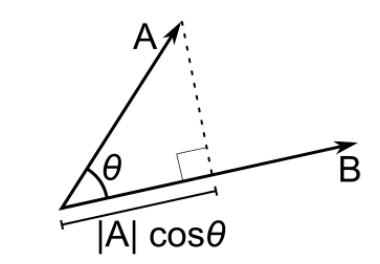
\includegraphics[width=0.4\linewidth]{cosine}	
\end{center}

Khi đó độ tương đồng giữa hai câu a và b sẽ được tính bằng giá trị cosine góc giữa 2 véc-tơ A và B :

\begin{center}
	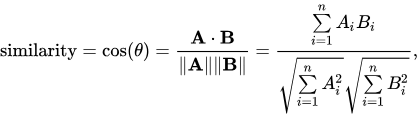
\includegraphics[width=0.7\linewidth]{similarity}
\end{center}
\hspace{20mm}Trong đó A và B lần lượt là các vector thuộc tính của 2 câu a và b. 

\hspace{20mm}||A|| là độ dài của vector thuộc tính A

\hspace{20mm}||B|| là độ dài vector thuộc tính B

Như vậy đầu ra của hàm tương tự này sẽ là giá trị trong khoảng [-1, 1], với giá trị -1 có nghĩa là hai véc-tơ so sánh hoàn toàn trái ngược nhau còn 1 sẽ là hoàn toàn giống nhau. Giá trị này sẽ là độ đo sự tương đồng giữa hai câu. Tuy nhiên trong thực tế đánh giá, giá trị này sẽ giao động trong khoảng [0, 1] 

Như vậy thuật toán tính độ tương tự này có thể được biểu diễn theo cách sau:

\textbf{Bước 1}: Chuyển đổi 2 câu thành hai véc-tơ

Mục đích của kĩ thuật này là ánh xạ câu văn sang một véc-tơ số thực để máy tính có thể sử dụng là đối số đầu vào để tính toán. Ở đây chúng ta có thể sử dụng một phương pháp khá phổ biến ở thời điểm hiện tại là phương pháp word2vec \cite{cia-word2vec}.

\textbf{Bước 2}: Tính khoảng cách giữa hai véc-tơ
Sau khi hai câu được biểu diễn dưới dạng véc-tơ, chúng ta hoàn toàn có thể tính độ tương đồng giữa chúng, một trong những phương pháp để tính độ tương đồng có thể kể đến như:
\begin{itemize}
	\item Độ đo cosine: Đây là một độ đo được dùng khá phổ biến khi muốn đánh giá độ tương đồng giữa hai véc-tơ ( đã được trình bày ở trên )
	\item Khoảng cách euclid: Đây cũng là một phương pháp được sửu dụng để đánh giá hai véct-tơ, công thức khoảng cách euclide \cite{cia-euclid} có dạng:
\end{itemize}
\begin{center}
	E(A, B) = $\sqrt{\sum_{i}^{n} (A_i - B_i) ^2}$
\end{center}

\hspace{20mm} Trong đó A, B lần lượt là véc-tơ biểu diễn của 2 câu, 
n là số chiều không gian để biểu diễn hai véc-tơ A và B

\hspace{20mm} Phương pháp euclide sẽ cho đánh giá tốt khi hai véc-tơ được biểu diễn dưới dạng liên tục hoặc dày đặc.

\subsection{Sử dụng máy tìm kiếm Google}

Đối với bài toán tìm kiếm những văn bản có nội dung tương đồng, đầu vào của quá trình sẽ có thể là những đoạn, hay câu văn sau khi đã được tiền xử lý. Và khi đó những câu, đoạn đó sẽ đóng vai trò như những từ khóa tìm kiếm. Google đã cung cấp một giao tiếp lập trình ứng dụng (API) để các lập trình viên có thể sử dụng chức năng tìm kiếm của Google
\begin{center}
	http://google.com.vn/search?q=Từ khóa
\end{center}

Kết quả trả về dưới dạng HTML, từ đó việc phân tích và trích xuất thông tin từ kết quả của máy tìm kiếm Google được thực hiện bằng cách phân tích kết quả HTML đó. 

Bên cạnh đấy, đối với máy tìm kiếm Google, chúng ta có thể khai thác thêm rất nhiều những cách truy xuất đặc biệt khi tủy chỉnh lại cụm "Từ khóa" sao cho phù hợp.

\section{Tìm kiếm nội dung tương đồng văn bản không cùng ngôn ngữ}

Mục tiêu của việc phát hiện tương tự nội dung văn bản không cùng ngôn ngữ là ước tính xem liệu hai đơn vị văn bản trong các ngôn ngữ khác nhau có thể hiện sự giống nhau hay không. Những phương pháp này thường sử dụng mô hình không gian véc-tơ.

Mô hình này kết hợp nhiều phương pháp và các mô hình học máy đã có bao gồm:
\begin{itemize}
	\item Cross-language Character N-Gram (CL- CnG) dựa trên mô hình của Mcnamee và Mayfield \cite{cia-ngram} để thực hiện so sánh hai đơn vị văn bản dựa trên so sánh cú pháp giữa chúng thông qua một mô hình n-gram. Nghiên cứu này thực hiện trên bộ dữ liệu được viết bằng các ngôn ngữ của các quốc gia châu Âu. Mô hình dựa trên xác suất xuất hiện của các n-gram thay vì các từ để truy xuất sự tương đồng. Dưới đây là bảng kết quả so sánh việc sử dụng n-gram và từ khi truy xuất độ trùng lặp giữa các hai ngôn ngữ tiếng Anh và Tây Ban Nha
	\begin{figure}[h]
		\centering
		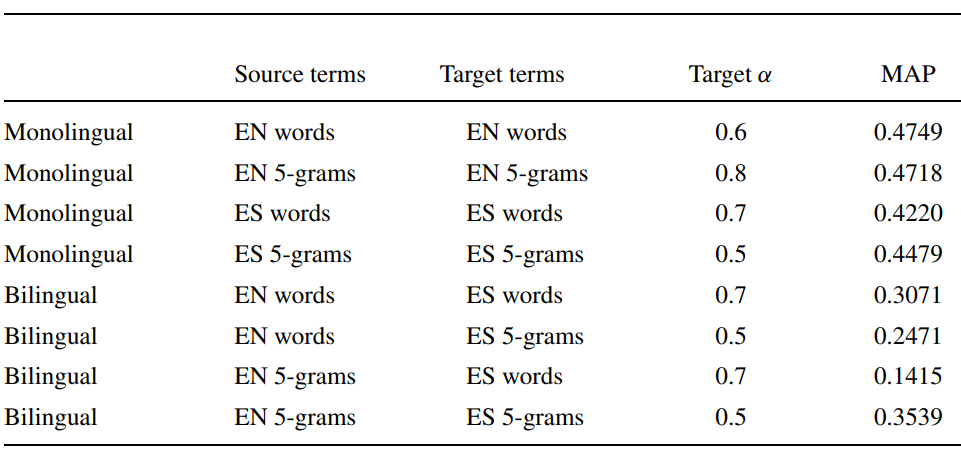
\includegraphics[scale=0.45]{ngram}
		\caption{Hình ảnh kết quả của phương pháp N-gram\cite{cia-ngram}}
	\end{figure}
	\item Dịch thuật và các mô hình tìm kiếm tương đồng trong cùng ngôn ngữ: Đây là mô hình có thể dễ dàng hình dung ra nhất vì những thuật toán cho sự tương đồng trong cùng ngôn ngữ đã đạt được những thành tựu nhất định. Mô hình sẽ dịch nội dung cần dịch thuật sang cùng một ngôn ngữ trước khi sử dụng những phương pháp so sánh đơn ngữ.
\end{itemize}

\section{Triển vọng phát triển của phương pháp đề xuất}

\textbf{Sự phát triển của công nghệ dịch thuật:}

Các công nghệ dịch của các công ty lớn như Google, Yandex thời điểm hiện tại đã cho những kết quả khá hoàn hảo và cung cấp những giao diện lập trình ứng dụng dễ dàng sử dụng (application programming interface) cho các nhà phát triển có thể sử dụng một cách dễ dàng, đây là một bước vô cùng quan trọng cho các mô hình tìm kiếm văn bản tương đồng không cùng ngôn ngữ. 

\noindent\textbf{Độ phức tạp của tiếng việt:}

Các bài toán về tìm kiếm nội dung tương đồng giữa các văn bản không cùng ngôn ngữ cũng đã được nghiên cứu với nhiều ngôn ngữ trên thế giới, tuy nhiên đối với tiếng Việt bài toán này còn chưa thực sự hấp dẫn được nhiều nghiên cứu và cũng chưa thực sự được đưa vào ứng dụng thực tế. Do đó đây có thể là một hướng đi khá khó khăn nhưng vẫn là một hướng đi triển vọng, cần được khai thác.

\chapter{Mô hình tìm kiếm đoạn nội dung tương đồng}
\label{chap:model}
Mục tiêu của phần này là xây dựng mô hình nhằm tìm kiếm đoạn nội dung tương đồng trên một tập cơ sở dữ liệu những văn bản đã có tuy nhiên lại không được viết cùng một ngôn ngữ. Các phương pháp, kiến trúc được ứng dụng dựa trên nghiên cứu cho những ngôn ngữ khác và phương pháp đề xuất sẽ được mô tả dưới đây.
\section{Yêu cầu bài toán}

Bài toán có thể được phát biểu đơn giản như sau:

\textbf{Đầu vào}: Một đoạn văn bản tiếng Việt được người dùng đưa vào dưới dạng thô, chưa được tiền xử lý (tách từ, bỏ các từ dừng, bỏ các dấu câu không cần thiết...)

\textbf{Đầu ra}: Các đoạn văn bản tiếng anh được sắp xếp theo có độ tương đồng về nội dung so với đoạn văn đầu vào 

Như đã được giới thiệu ở \textbf{Chương \ref{chap:intro}}, khóa luận được nghiên cứu để truy xuất những đoạn văn bản tiếng Anh có nội dung tương đồng với đoạn văn bản tiếng Việt đầu vào. Mục tiêu khóa luận hướng đến đóng góp cho việc phòng chống đạo văn, mô hình được đề xuất sẽ tìm kiếm ra những đoạn văn bản có nội dung tương đồng có khả năng đã bị sao chép, từ đó ta có thể áp dụng những phương pháp so sánh chi tiết từng câu. Với trường hợp cần những chuyên gia để xác định đạo văn, công việc cũng sẽ giảm đi rất nhiều vì họ chỉ cần so sánh đoạn văn bản đầu vào với những văn bản đã được mô hình truy xuất.

\section{Mô hình đề xuất giải quyết bài toán}

Trong phần này, mô hình để tìm kiếm đoạn nội dung không cùng ngôn ngữ sẽ được giới thiệu, bên cạnh đó tôi cũng sẽ trình bày những thuật toán quan trọng để xây dựng lên mô hình này.

\subsection{Kiến trúc mô hình}

\begin{figure}[h]
	\centering
	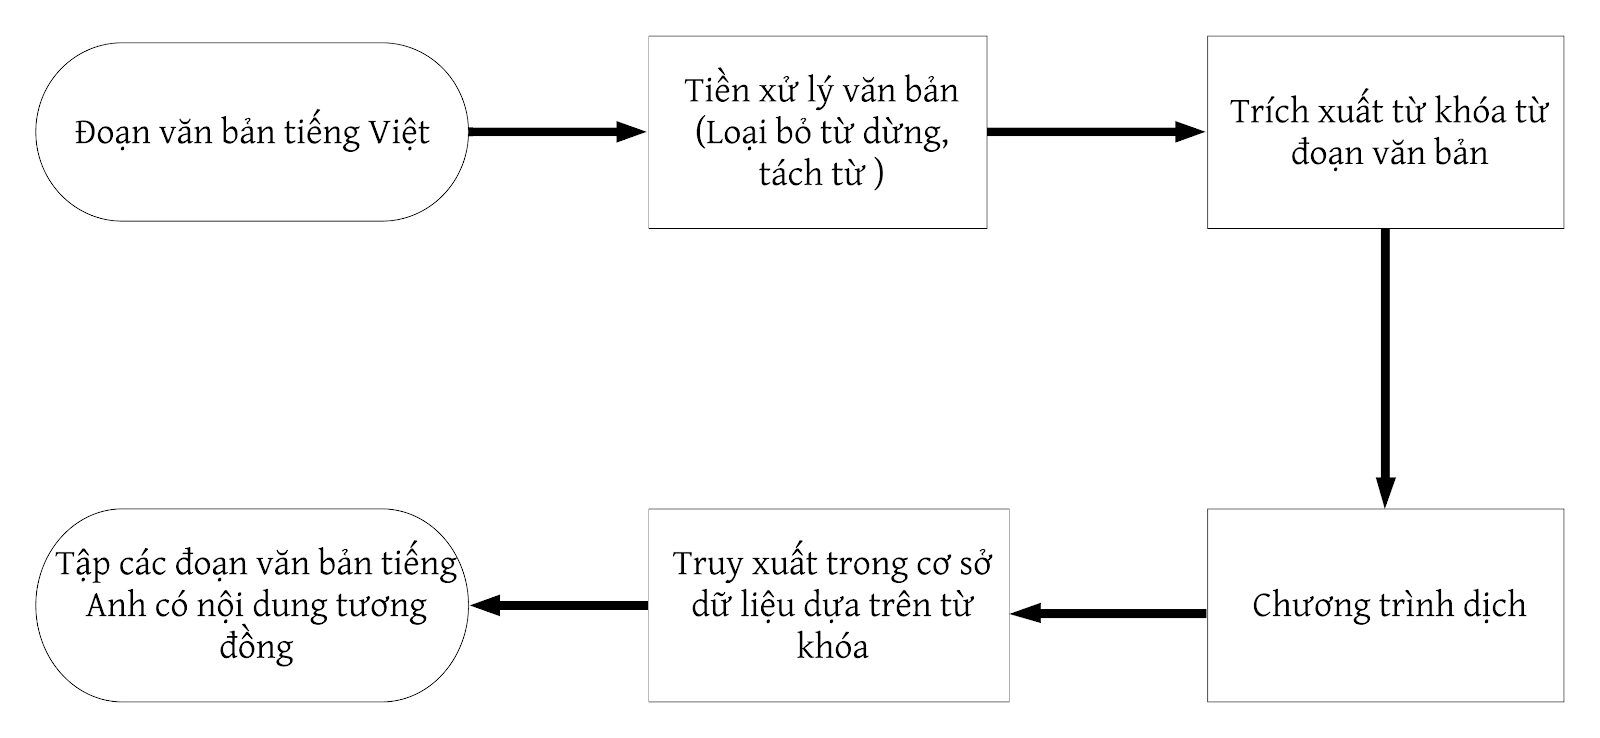
\includegraphics[scale=0.25]{architecture}
	\caption{Hình ảnh mô hình kiến trúc xử lý tìm kiếm trong đoạn văn tưởng đồng không cùng ngôn ngữ}
\end{figure}
Trong bài toán nghiên cứu của mình, tôi đề xuất mô hình tìm kiếm đoạn nội dung tương đồng với những mô-đun chính như sau:
\begin{itemize}
	\item Mô-đun tự động thu thập văn bản được viết bằng tiếng Anh để xây dựng cơ sở dữ liệu.
	\item Mô-đun tiền xử lý văn bản.
	\item Mô-đun trích xuất từ khóa.
	\item Mô-đun truy xuất văn bản tương đồng trong cơ sở dữ liệu
\end{itemize}

\subsection{Mô-đun tiền xử lý văn bản }
\hspace{10mm}\textbf{Loại bỏ nhiễu}

Những dữ liệu thu thập phần lớn là những dữ liệu được thu thập từ dữ liệu web, do đó để có một đầu ra hợp lý ( tạo ra nội dung trang web dưới dạng văn bản) cần phải loại bỏ những kí tự không mong muốn bị lẫn vào như ví dụ sau đây:

\begin{figure}[h]
	\centering
	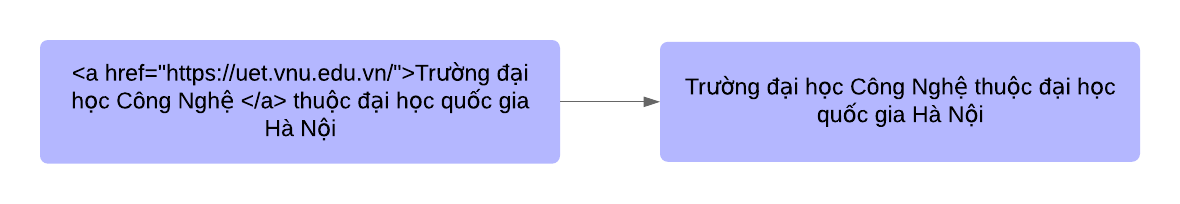
\includegraphics[scale=0.9]{remove_noise}
	\caption{Hình ảnh mô hình kiến trúc xử lý tìm kiếm trong đoạn văn tưởng đồng không cùng ngôn ngữ}
\end{figure}

Trong quá trình thực nghiệm, nhận thấy phần lớn các nhiễu xuất hiện thường do lẫn các thẻ HTML vào trong dữ liệu thu thập, do đó các  nhiễu này có thể loại bỏ bằng các biểu thức chính quy.

Sau bước trên chúng ta có thể đã có được một mẫu văn bản khá dễ đọc , tuy nhiên dữ liệu đầu ra ở đây vẫn đang ở dạng thô, để phục vụ việc trích xuất từ khóa cho những văn bản tiếng Việt thì chúng ta cần thêm một công đoạn là tách từ, công đoạn này sẽ được nói ở phần tiếp theo.

\textbf{Tách từ trong câu}

Đối với văn bản tiếng Anh việc tách từ rất đơn giản so với tiếng Việt, mỗi từ trong tiếng Anh được phân tách với nhau thông qua dấu " " (cách) còn với tiếng Việt, một từ có thể được cấu tạo từ một hoặc nhiều tiếng (từ phức). Để có thể tạo ra một bộ từ khóa hợp lý thì việc tách từ có ý nghĩa khá quan trọng, sau đây là một ví dụ về tầm quan trọng của việc tách từ:


\begin{figure}[h]
	\centering
	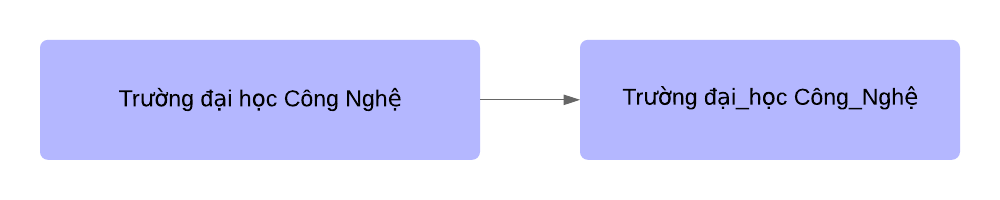
\includegraphics[scale=0.9]{word_token}
	\caption{Hình ảnh ví dụ một trường hợp tách từ tiếng Việt}
\end{figure}

Có thể nhận thấy nếu giữ nguyên bản của câu trên thì việc trích xuất từ khóa sẽ gặp phải rất nhiều khó khăn. Với từ phức "đại học" nếu tách ra làm hai từ đơn là "đại" và "học" thì hai từ độc lập này vẫn có nghĩa nhưng nếu những từ đơn này trở thành từ khóa thì có thể gây nhiều nhiễu khi dịch thuật vì nó không thể hiện rõ nghĩa của từ trong bối cảnh của văn bản: 

\begin{table}[h]
	\centering
	\caption{Bảng ví dụ các trường hợp hạn chế khi dịch thuật}
	\begin{tabular}{|l|c|}
		\hline
		\textbf{Tiếng Việt}             & \textbf{Tiếng Anh} \\ \hline
		Đại học                         & University  \\ \hline
		Đại															& Greate			\\ \hline
		Học                             & Learn 			\\ \hline
	\end{tabular}	
\end{table}

Với ví dụ trên có thể thấy tầm quan trọng của công đoạn tách từ đối với những văn bản tiếng Việt. Có thể nói đây là bước tiền đề để có thể xây dựng bộ từ khóa đại diện cho văn bản.

\textbf{Loại bỏ từ dừng}

Từ dừng xuất hiện cả trong tiếng Việt cũng như tiếng Anh, đây là những từ xuất hiện trong các văn bản với tần suất cao nhưng lại không chứa nhiều ý nghĩa. Các từ dừng trong tiếng Việt hay xuất hiện như thì, là, đó, vậy,... trong tiếng Anh như this, that, of…
Với công đoạn này chúng ta có một phương pháp đơn giản là xây dựng một bộ từ điển chứa các từ dừng và lọc văn bản đầu vào và lọc bỏ đi những từ dừng đó.

Mô-đun tiền xử lý văn bản được áp dụng cho cả hai phía văn bản tiếng Việt đầu vào ( mục đích truy vấn ) và văn bản tiếng Anh  ( mục đích để xây dựng cơ sở dữ liệu truy xuất ). Tuy nhiên tùy với từng loại ngôn ngữ mô-đun tiền xử lý văn bản có những tùy chỉnh riêng để có thể đưa ra những kết quả hợp lý nhằm loại bỏ những từ dừng không mong muốn.

\subsection{Mô-đun thu thập văn bản được viết bằng tiếng Anh}

Như đã được giới thiệu, mô-đun này mục đích là tự động xây dựng cơ sở dữ liệu để truy xuất đưa ra kết quả những tập văn bản tiếng Anh có độ tương đồng với văn bản tiếng Việt đầu vào.

Mô-đun này trực tiếp thu thập dữ liệu từ những trang web đã được định nghĩa trước, những văn bản thu thập về sẽ được lưu trữ theo những thể loại tương ứng với mục đích tăng độ chính xác cho mô-đun trích xuất từ khóa với phương pháp TF-IDF.

Mô-đun sẽ tự động cập nhật để xây dựng cơ sở dữ liệu truy xuất từng ngày để có thể luôn tự động cập nhật cơ sở dữ liệu mới nhất. Mô-đun này sử dụng một chương trình để lấy được cây mô hình đối tượng tài liệu (DOM) của các trang web mục tiêu, từ đó phân tích các nút trong cây DOM để có thể trích xuất những thông tin nội dung của văn bản được thu thập. Những văn bản được thu thập sẽ đi qua mô-đun tiền xử lý, tại đây văn bản sẽ được tách đoạn, làm sạch, tách từ \dots

Cây mô hình đối tượng tài liệu của trang web rất đa dạng cho từng trang web, do đó việc trích xuất dữ liệu từ chúng vẫn chưa thực sự đi đến một cách tự động.


\begin{figure}[h]
	\centering
	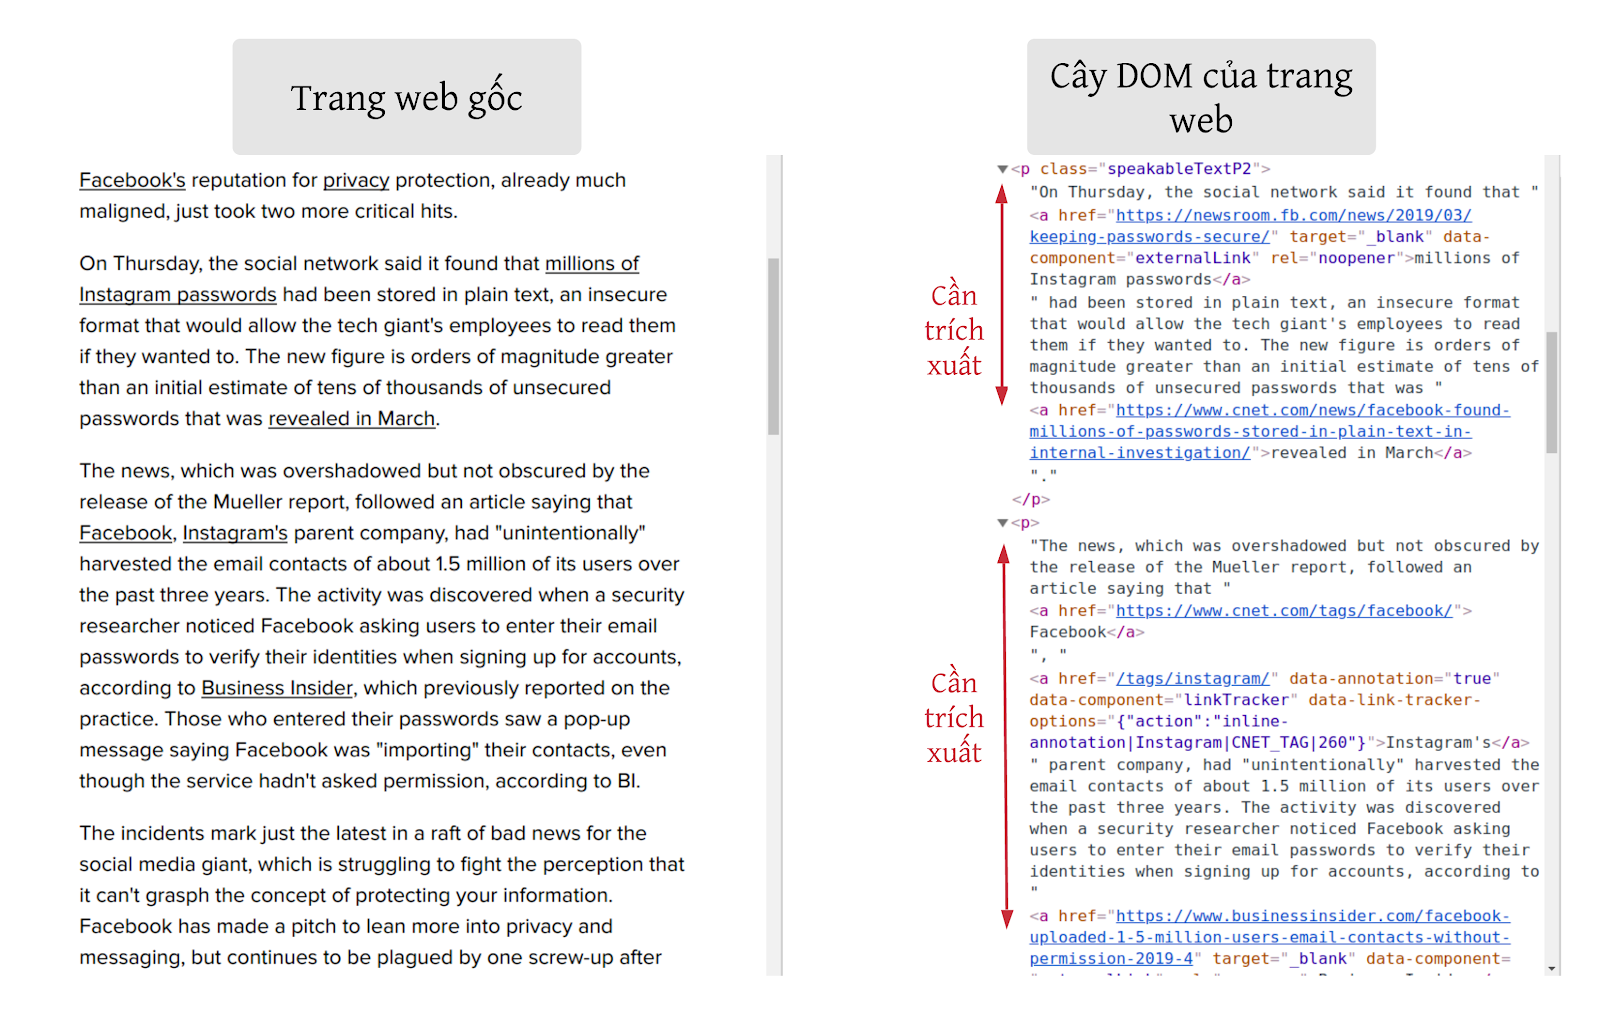
\includegraphics[scale=0.3]{DOM-tree}
	\caption{Hình ảnh cây mô hình đối tượng tài liệu của một trang web trong thực tế	}
\end{figure}

Sự đa dạng của những trang web này khiến cho mô-đun phải tùy chỉnh cho từng nguồn vì phương pháp thu thập dữ liệu hiện tại là dựa trên cấu trúc cây DOM để  có  thể lấy ra những phần nội dung cần thiết. 

\newpage
\subsection{Mô-đun trích xuất từ khóa}

Trong khóa luận lần này, tôi xin trình bày về phương pháp mà khóa luận sử dụng là phương pháp tiếp cận theo hướng thống kê:

Hướng tiếp cận này thường sử dụng thông tin về tần số thống kê tần suất để chọn ra các từ khóa quan trọng. Thuật toán trích xuất từ khóa dựa trên tần số xuất hiện cục bộ và toàn cục TF-IDF \cite{cia-tfidf}  . Nguyên lý hoạt động của thuật toán này dựa trên việc xác định độ quan trọng của một từ : Độ quan trọng sẽ tăng lên khi từ xuất hiện nhiều trong văn bản và giảm xuống khi từ đấy cũng xuất hiện trong nhiều văn bản khác.

\textbf{TF} : Tần số xuất hiện của một từ trong văn bản
\begin{center}
	TF(t, d) = $\mbox{\Huge}\frac{f(t, d)}{ \sum_{t' \in D} f(t', D)}$	
\end{center}

Tỉ lệ này là số lần xuất hiện của một từ trên tổng số từ của văn bản, giá trị này nằm trong khoảng [0, 1]

\textbf{f(t, d)}  : Số lần xuất hiện của từ t trong văn bản d

\textbf{$\sum_{t' \in D} f(t', D)$} : Tổng số từ trong văn bản d 


\textbf{IDF}: Tần số nghịch của một từ trong tập văn bản

\begin{center}
	IDF (t, D) = $\log{(\frac{|D|}{|{ d \in D; t \in d }|})}$
\end{center}

|D| : Tổng số văn bản trong D

$|{ d \in D; t \in d }|$ :  Số văn bản chứa từ nhất định. Nếu từ t không xuất hiện trong bất cứ văn bản nào thì mẫu số bằng 0, do đó công thức này có thể thay đổi mẫu thành dạng 1 + |{ d  D; t  d }|

Từ đó ta xây dựng được công thức:
\begin{center}
	TF-IDF(t, d, D) = TF(t, d) $\times$ IDF(t, D)	
\end{center}

Những từ có giá trị TF-IDF cao là những từ xuất hiện nhiều trong văn bản đang xét và xuất hiện ít trong các văn bản khác nhớ đó ta có thể lọc ra những từ có giá trị cao để xây dựng bộ từ khóa.

Mô-đun trích xuất từ khóa của cả tiếng Anh cùng được sử dụng chung phương pháp TF-IDF (term frequency - inverse document frequency) để trích xuất từ khóa. Phương pháp này đòi hỏi cần phải có những tập văn bản đã có sẵn để có thể tính toán được IDF, do đó bộ lưu trữ của kiến trúc sẽ phải tồn tại những tập các đoạn văn bản tiếng Việt và tiếng Anh.

Những bộ từ khóa của văn bản tiếng Anh sau khi được trích xuất sẽ tiếp tục được sử dụng như một cơ sở dữ liệu truy xuất do đó chúng cũng sẽ được giữ lại tại bộ lưu trữ của mô hình kiến trúc.

Với bộ dữ liệu là các đoạn văn bản, mô-đun trích xuất từ khóa sẽ đóng góp hai việc quan trọng cho mô hình gồm :
\begin{itemize}
	\item Trích xuất từ khóa của đoạn văn tiếng Việt nhằm tạo ra đối số đại diện cho văn bản đầu vào để truy xuất trong mô-đun truy xuất những đoạn văn tương đồng. Với mỗi văn bản đầu vào, nếu sử dụng hoàn toàn phương pháp TF-IDF sẽ mất một lượng tính toán cũng như thời gian khá lớn vì phải tính lại toàn bộ IDF của một tập các văn bản tiếng Việt. Do đó trong trường hợp tiếng Việt, tôi đề xuất sử dụng TF và sử dụng một từ điển các từ dừng để hạn chế việc xuất hiện trong bộ từ khóa những từ ngữ không có giá trị ca. 
	\item Trích xuất từ khóa từ tập các đoạn văn tiếng Anh nhằm xây dựng cơ sở dữ liệu các đại diện cho việc truy xuất, mỗi bộ từ khóa sẽ đại diện cho các đoạn văn tiếng Anh tương ứng, mô-đun truy xuất đoạn văn bản tương đồng sẽ sử dụng các đại diện này như một bộ dữ liệu để truy xuất thông qua các đại diện là tập từ khóa đã được trích xuất.
	\begin{figure}[h]
		\centering
		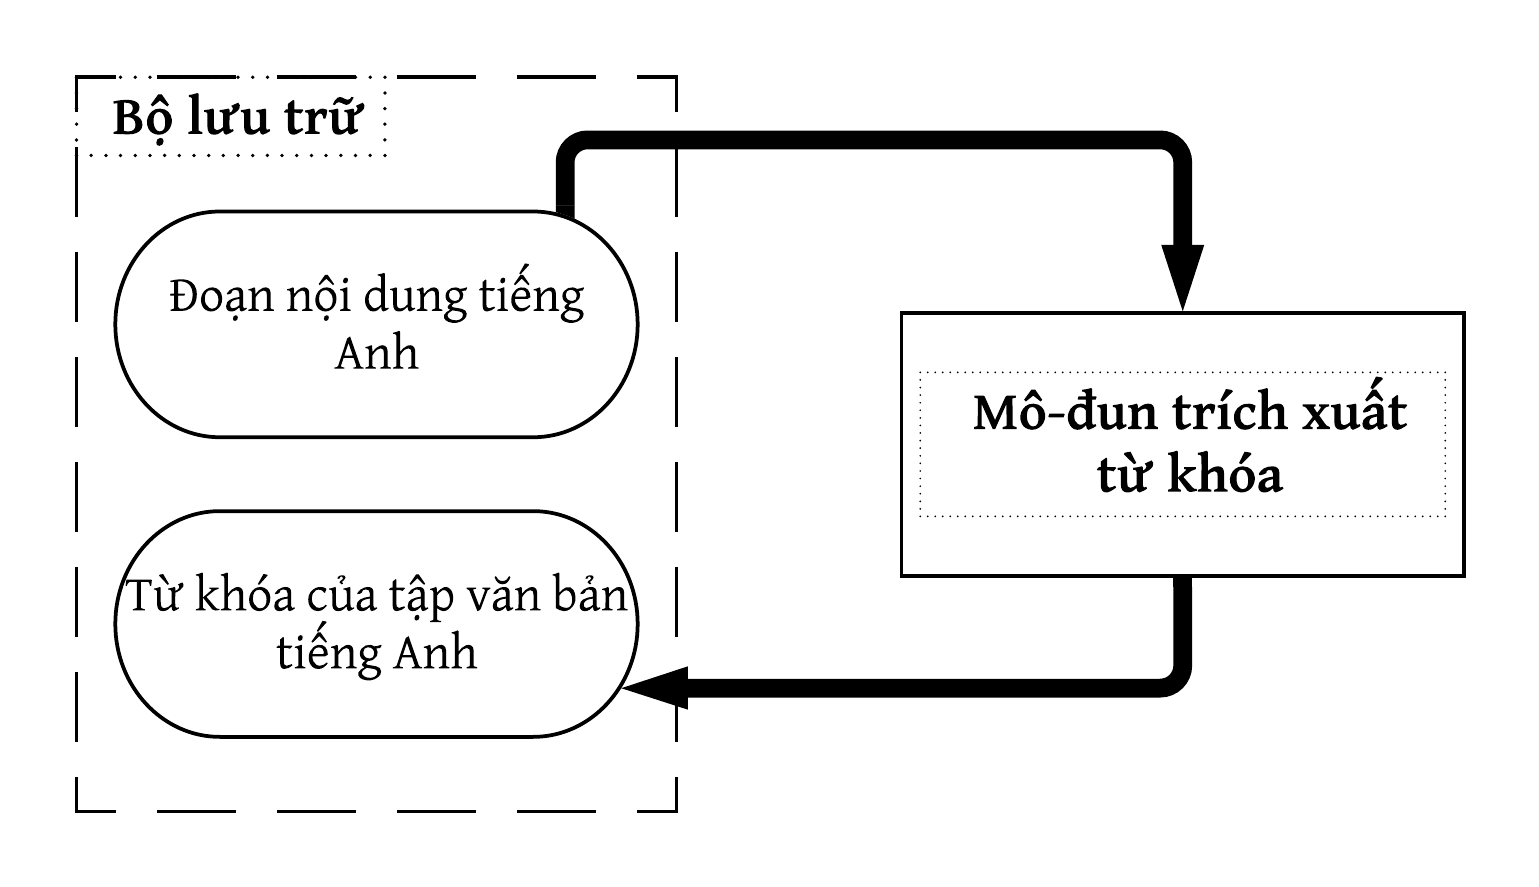
\includegraphics[scale=0.9]{tfidf}
		\caption{Hình ảnh tập các đoạn văn bản tiếng Anh được trích xuất từ khóa tương ứng sử dụng phương pháp TF-IDF}
	\end{figure}
\end{itemize}

\subsection{Mô-đun truy xuất những đoạn văn bản tương đồng}

Tại mô-đun này, tôi đề xuất hai phương pháp tìm kiếm sự tương đồng nội dung dựa theo hàm băm (hash-based search) tìm kiếm với các đại diện là các tập từ khóa và sử dụng so sánh các ma trận véc-tơ được ánh xạ từ những bộ từ khóa thông qua một mô hình không gian véc-tơ.

\subsubsection{Tìm kiếm dựa trên hàm băm (hash-based search):}

\textbf{Độ đo tương tự Jaccard:}

Đầu tiên chúng ta sẽ phải nói về phương pháp đo độ tương tự giữa hai văn bản. Như đã đề cập ở chương 2, ta có thể tính độ tương tự của hai văn bản bằng cách chuyển đổi chúng sang dạng véc-tơ và tính toán độ tương đồng, tuy nhiên để chuyển đổi một văn bản sang một véc-tơ tốn khá nhiều công sức tính toán, do đó phương pháp tính toán độ tương tự giữa hai văn bản lần này tôi muốn trình bày là phương pháp độ đo Jaccard \cite{cia-jaccard}. Độ đo Jaccard giữa hai tập hợp A và B được tính dựa trên tỉ lệ giữa số lượng các phần tử giao nhau giữa A và B trên số lượng phần tử của hợp giữa A và B.

Độ đo này được biểu diễn bởi công thức sau:

\begin{center}
	J (A, B) = $\frac{|A \bigcap B|}{| A \bigcup B|}$

	Tỉ lệ này nằm trong khoảng 0\% - 100\%

	$|A \bigcap B|$ : Số lượng phần tử trùng nhau của hai tập A và B
	
	$|A \bigcup B|$ : Số lượng phân tử hợp của hai tập A và B 

\end{center}

Bài toán này có thể được minh họa bằng ví dụ :

Với hai câu
\begin{itemize}
	\item Ai là hiệu trưởng trường đại học Công Nghệ.
	\item Ai là người đứng đầu trường đại học Công Nghệ. 
\end{itemize}

Tách mỗi câu thành hai tập hợp có phần tử là các tiếng trong câu

Ta có thể mô phỏng lại phương pháp Jaccard \cite{cia-jaccard} bằng hình vẽ :

\begin{figure}[h]
	\centering
	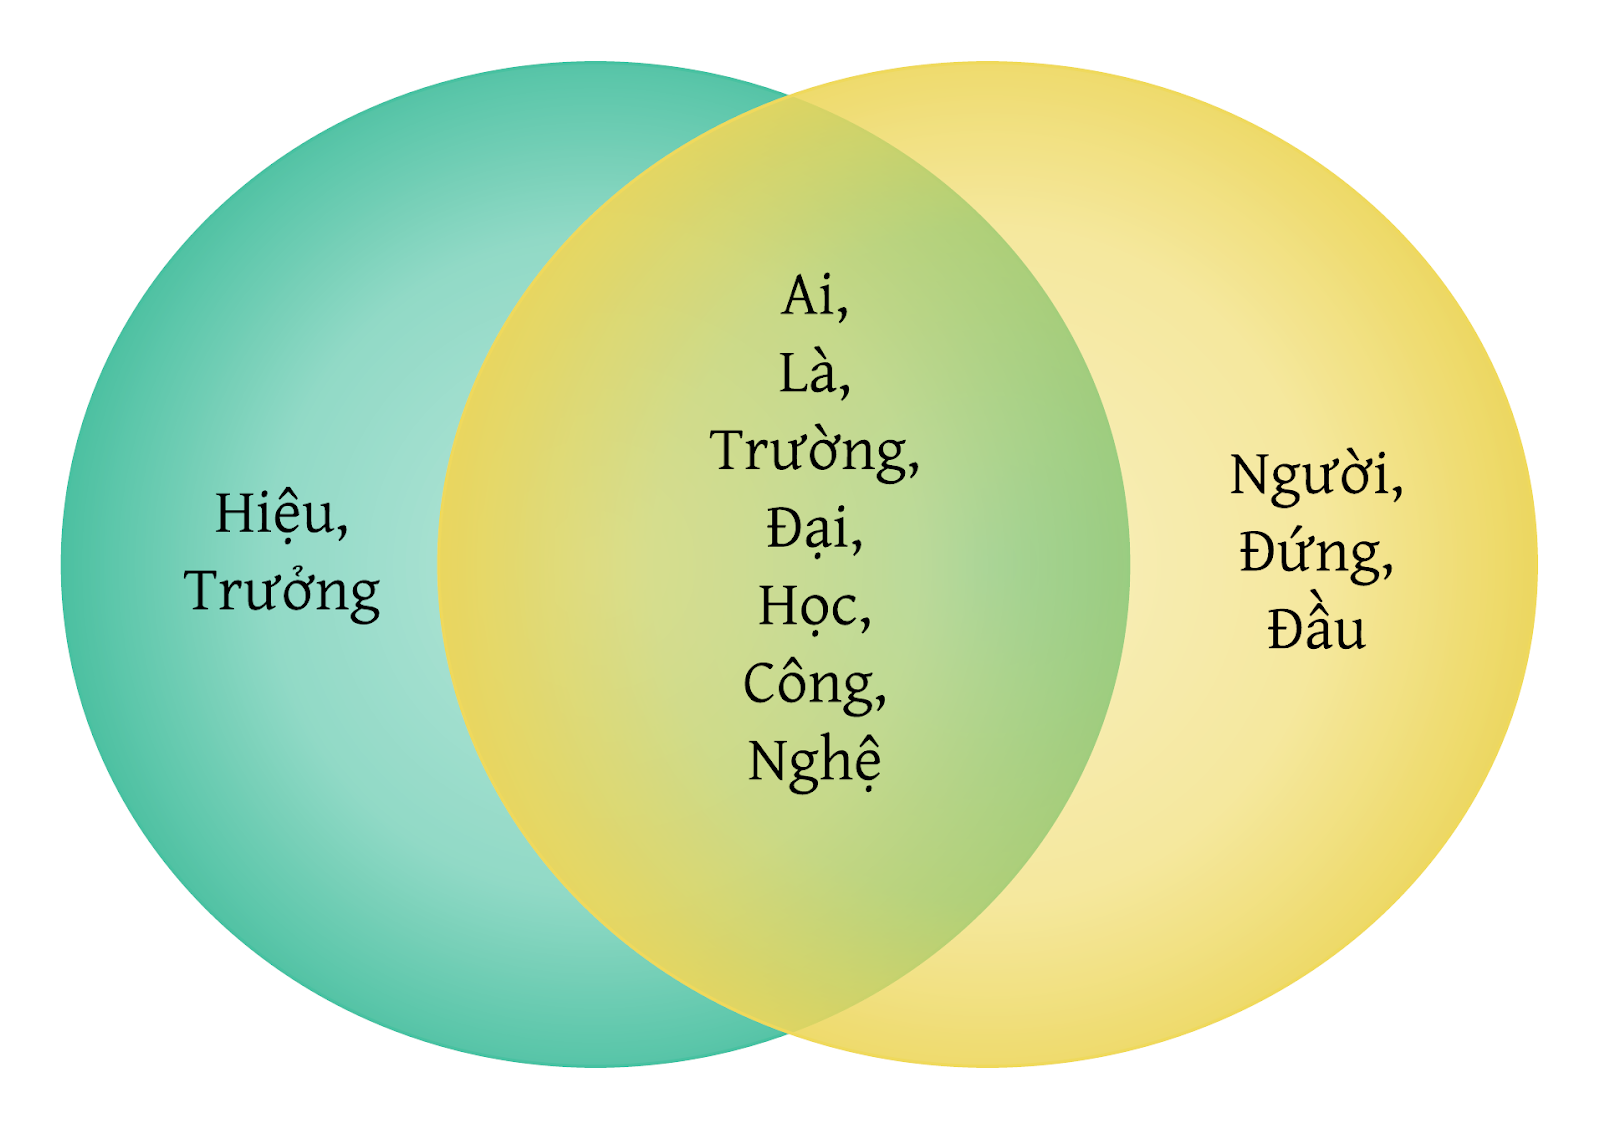
\includegraphics[scale=0.3]{jaccard_exp}
	\caption{Hình ảnh sơ đồ venn giữa phần tử tập hợp hai câu}
\end{figure}

Với ví dụ này tôi đang lấy dựa trên đơn vị là tiếng, các câu đầu vào chưa được tách từ. Có thể thế số lượng phần tử giao nhau là 12 phần tử, số lượng phần tử hợp là 17. Như vậy độ đo Jaccard giữa hai câu A và B là $\frac{12}{17}$ $\approx$ 0.7


\noindent \textbf{Hàm băm MinHash và băm địa phương nhạy cảm (Locality Sensitive Hashing):}

Với phương pháp dựa vào độ đo Jaccard đã đề cập phần trên, ta phải 
so sánh từng cặp văn bản, tính tổng số phần tử chung của mỗi cặp trước trước khi tính ra được độ đo Jaccard. Với một lượng lớn cơ sở dữ liệu cần truy xuất thì lượng tính toán như vậy là quá cao

Để giải quyết vấn đề này, khóa luận sẽ được cài đặt một hàm băm như được đề xuất trong \cite{cia-cross}. Các văn bản sẽ được biểu diễn dưới một tập các số nguyên, tập này được gọi là dấu vân tay (fingersprints).


Sử dụng hàm băm địa phương nhạy cảm (Locality Sensitive Hashing) để cài đặt cho hướng tìm kiếm tương đồng nội dung giữa hai loại văn bản tiếng Việt và tiếng Anh. Chúng ta có thể sử dụng trực tiếp hàm băm MinHash để biến đổi những tập từ khóa của các văn bản sang dạng vân tay (fingersprints).

Trong khóa luận này tôi xin đề xuất phương pháp sử dụng trực tiếp hàm băm MinHash để đánh giá độ đo Jaccard giữa hai văn bản \cite{cia-mining}. MinHash là một hàm băm thuộc họ hàm băm địa phương nhạy cảm ( Locality Sensitive Hashing) \cite{cia-lsh}


Hàm băm MinHash xuất phát từ ý tưởng ánh xạ mỗi văn bản bằng một dấu vân tay (fingersprints) và thông qua nó để so sánh độ tương đồng giữa các văn bản.


Thuật toán của hàm băm MinHash có dạng:

\begin{algorithm}[H]
	\SetAlgoLined
	MinHash(A, D) :

	min $\gets$ + $\infty$
	
	Duyệt từng phần tử i trong A:
		
	\hspace{10mm}j $\gets$ trị số của i trong hoán vị D
		
	\hspace{10mm}Nếu j < min
	
	\hspace{20mm}min = j
	
	Trả về min
	\caption{Thuật toán MinHash}
\end{algorithm}
Trong đó A là một tập hợp phần tử cần lấy hoán vị

D là hoán vị ngẫu nhiên đầu vào 
		
\newpage
Ví dụ về mô hình xây dựng dấu vân tay (fingersprints) dựa trên hàm băm MinHash :

Cho 2 đoạn văn bản a và b, mỗi văn bản được biểu diễn bằng các tập từ khóa tương ứng là A, B. Khi đấy ta có thể xây dựng một từ điển từ D = A $\bigcup$ B. Lấy ngẫu nhiên các hoán vị của tập D, khi đó mỗi hoán vị có thể tạo ra một phần của dấu vân tay của A cách sử dụng hàm băm MinHash với đầu vào là tập phần tử của A và hoán vị D ( tương ứng cho văn bản B ). Cứ như vậy sau n hoán vị, chúng ta có được một mảng n phần tử các chỉ số được coi là dấu vân tay đại diện cho văn bản. Có một lưu ý trong việc xây dựng hàm MinHash này là về số lượng hoán vị, độ chính xác sẽ tăng khi số lượng hoán vị tăng theo số lượng hoán vị tuy nhiên sẽ phải đánh đổi về khả năng xử lý sẽ tốn thời gian hơn.

Sau đây sẽ là phần chứng minh tại sao có thể nói rằng phương pháp hàm băm có thể thay thế độ đo Jaccard:

Giả sử ta có một tập A' $\subset$ A, một tập hoán vị P : A $\subset$ P và B $\subset$ P, khi đó tỉ lệ để  một phần tử trong A' có chỉ số nhỏ nhất trong P là $\frac{1}{|A|}$ , như vậy xác suất để hàm băm MinHash của A và B bằng nhau chính là xác suất mà một phần tử bất kì trong tập A $\bigcap$ B trở thành phẩn tử có chỉ số nhỏ nhất trong tập A $\bigcup$ B - tương đương với công thức :
\begin{center}
	$\frac{|A \bigcap B|}{| A \bigcup B|}$
\end{center}

Nhận thấy đây cũng chính là công thức của độ đo tương tự Jaccard cho hai tập hợp phần tử. Như vậy với việc sử dụng MinHash, chúng ta vẫn giữ được tính chất của độ đo tương tự Jaccard mà đã giảm đi một lượng lớn tính toán.

Mô-đun trích xuất từ khóa phía trên đã xây dựng được một cơ sở dữ liệu tập từ khóa tương ứng cho những đoạn văn bản tiếng Anh, bằng cách ánh xạ những tập từ khóa trong cơ sở dữ liệu đó qua hàm băm MinHash chúng ta có một bảng băm cho các vân tay (fingersprints) với nhiệm vụ là cơ sở dữ liệu để truy xuất. Khi đó với một văn bản tiếng Việt đầu vào sẽ trích xuất bộ từ khóa sau khi đã được tiền xử lý, bộ từ khóa sẽ là đối số đầu vào của hàm băm MinHash.

\begin{figure}[h]
	\centering
	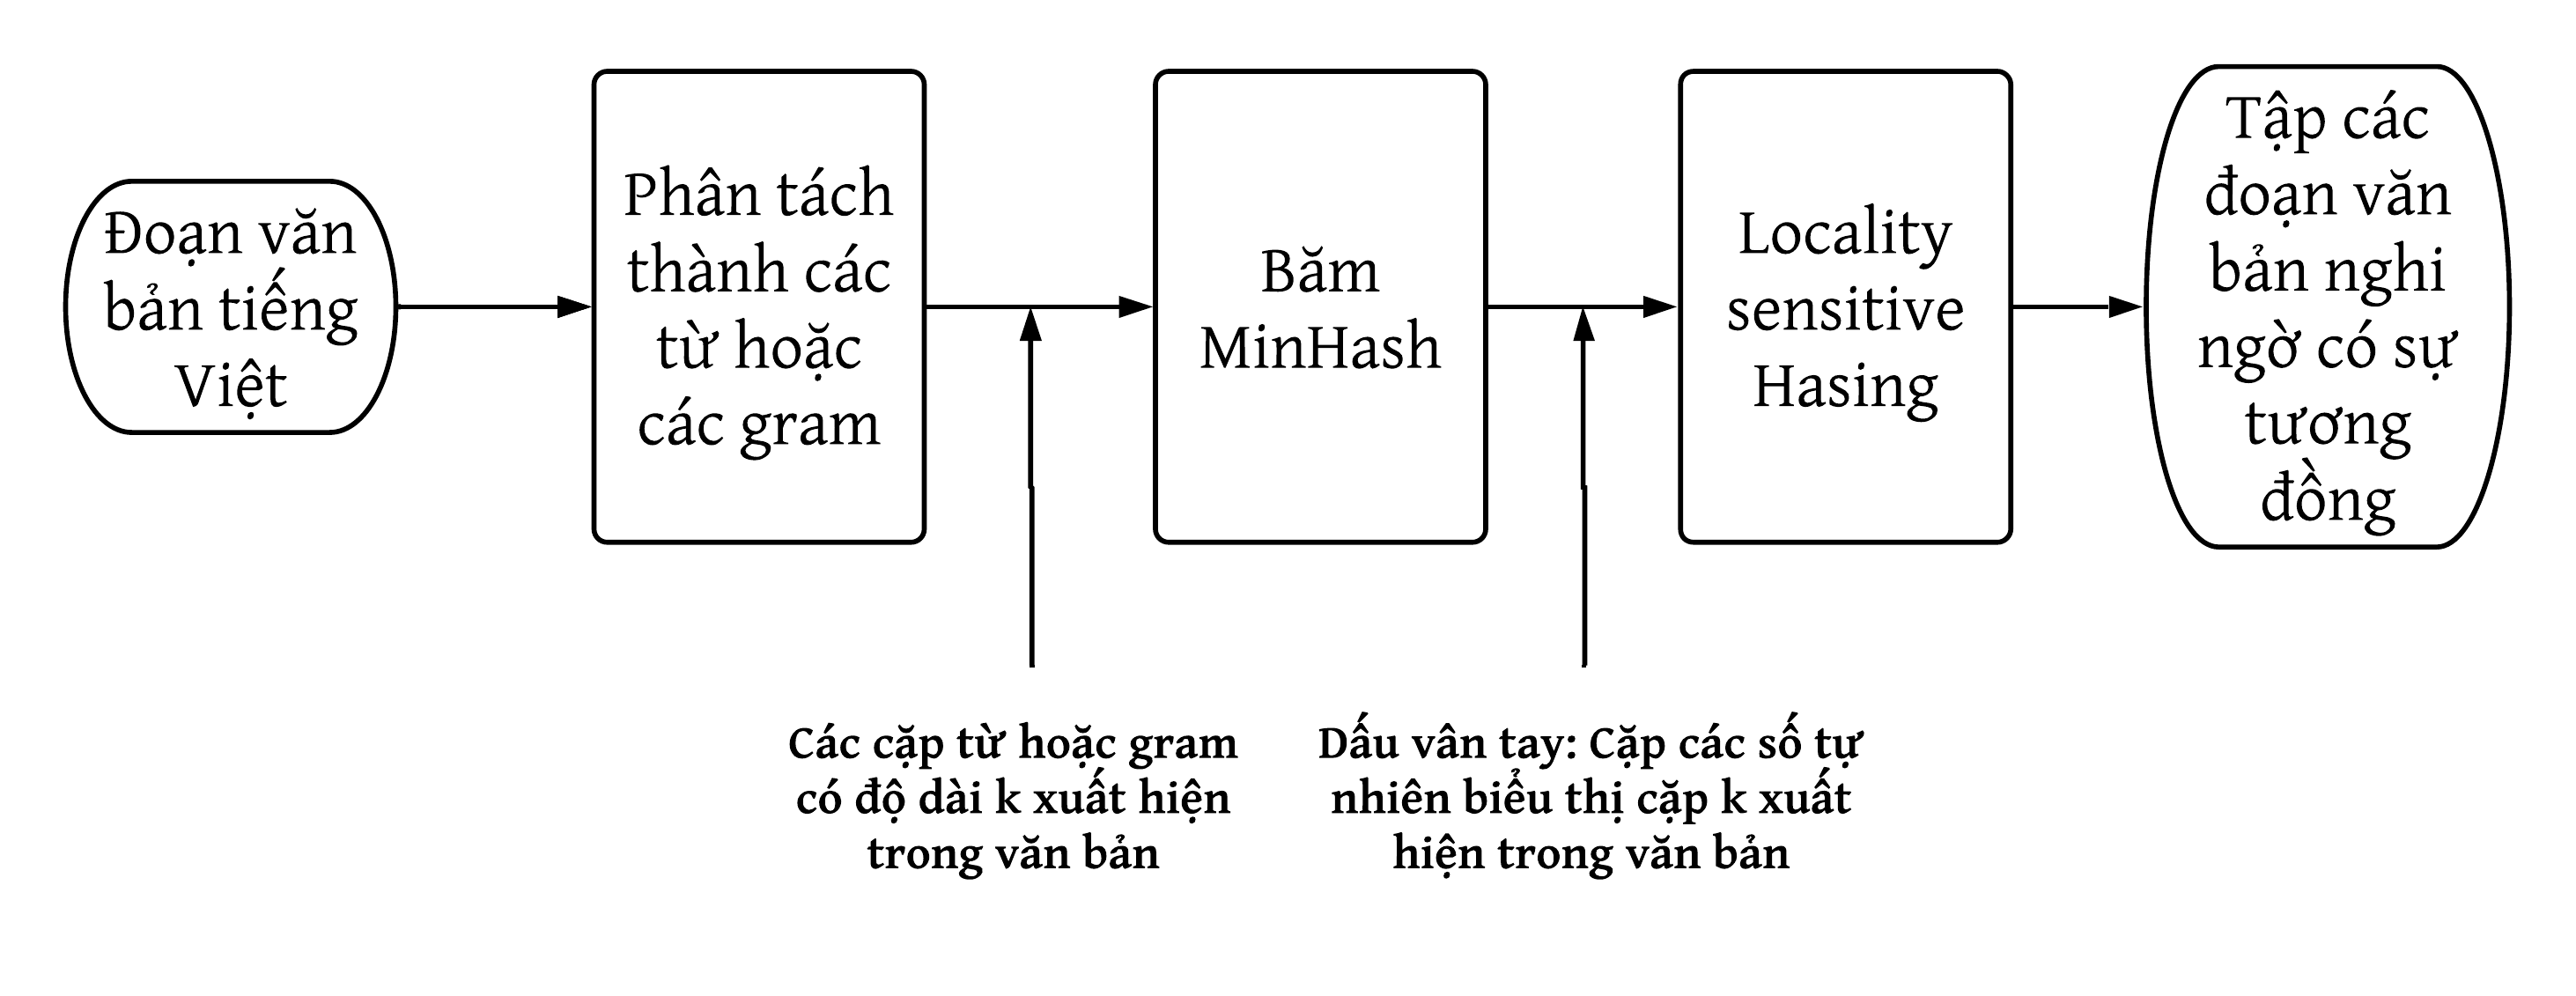
\includegraphics[scale=0.6]{lsh_total}
	\caption{Hình ảnh tổng quan về phương pháp băm}
\end{figure}

\subsubsection{Tìm kiếm thông qua mô hình không gian véc-tơ:}
Phương pháp này được để xuất dựa trên những thực nghiệm về sự phức tạp ngữ nghĩa của tiếng Việt, khi sử dụng chương trình dịch để đưa bộ từ khóa về cùng ngôn ngữ có thể gây ra những nhập nhằng

\begin{table}[H]
	\centering
	\caption{Bảng ví dụ trường hợp nhập nhằng với chương trình dịch}
	\begin{tabular}{|l|l|lll}
	\cline{1-2}
	Tiến Viêt                 & Bản dịch tiếng Anh &  &  &  \\ \cline{1-2}
	\multirow{3}{*}{Khám phá} & Discover           &  &  &  \\ \cline{2-2}
														& Expose             &  &  &  \\ \cline{2-2}
														& Explore            &  &  &  \\ \cline{1-2}
	\end{tabular}
\end{table}

Từ bảng ta thấy nếu từ "khám phá" trở thành từ khóa của văn bản đầu vào thì rất có thể sau khi qua chương trình dịch sẽ có nhiều kết quả trả về, sự nhập nhằng ở đây có thể khiến phương pháp tìm kiếm dựa vào hàm băm gặp những hạn chế vì nó chỉ dựa hoàn toàn trên ngữ pháp.

\noindent\textbf{Đề xuất ý tưởng dựa trên ngữ nghĩa của từ vựng}

Từ m từ khóa đại diện cho các đoạn văn bản, ánh xạ thông qua một mô hình không gian từ vựng n chiều ta sẽ xây dựng được một ma trận m $\times$ n. Ma trận này sẽ là đại diện mới cho các đoạn văn bản trong phương pháp thông qua mô hình không gian véc-tơ :
\begin{figure}[h]
	\centering
	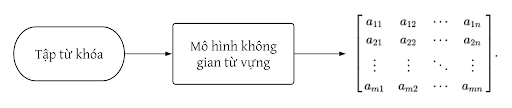
\includegraphics[scale=0.8]{vectornize}
	\caption{Hình ảnh chuyển đổi từ tập từ khóa sang ma trận véc-tơ}
\end{figure}

Ma trận kết quả trong Hình có càng hàng đại diện cho những véc-tơ biểu diễn của các từ khóa khi được ánh xạ qua mô hình không gian từ vựng.

Đối với bộ từ khóa của văn bản tiếng Việt đầu vào ( kết quả của mô-đun trích xuất từ khóa) cần thêm một bước dịch thuật sang tiếng Anh trước khi cho qua mô hình không gian từ vựng để tạo ra ma trận véc-tơ tương ứng. Bộ từ khóa của những văn bản tiếng Anh cũng phải được đưa cùng qua một mô hình không gian từ vựng tương tự thì mới tạo ra được những kết quả có tính tương đương.

Như vậy văn bản tìm kiếm và những văn bản được tìm kiếm đã được biểu diễn dưới dạng một ma trận. Công việc của mô hình sẽ là tính giá trị so sánh cặp giữa các ma trận để tìm ra những cặp ma trận độ tương tự cao nhất.

Gọi hai ma trận m $\times$ n ( trong trường hợp này m sẽ tương ứng số từ khóa, n tương ứng với số chiều véc-tơ của mô hình không gian từ vựng ) cần so sánh là A và B ,  trong trường hợp này ta có thể hiểu A là ma trận biểu diễn cho văn bản tiếng Việt, B là một ma trận biểu diễn cho một văn bản tiếng Anh, khi đấy ta tính độ tương tự cosine các cặp giữa hai ma trận này ta sẽ được ma trận kết quả R. Phương pháp này tính độ tương tự cosine của các hàng ma trận A với các hàng của ma trận B \cite{cia-pairwise}. Từ đó ma trận kết quả R là một ma trận m$\times$m với mỗi hàng là giá trị độ tương tự cosine của một véc-tơ từ khóa ma trận A so với các véc-tơ từ khóa của ma trận B. 

Ma trận kết quả R với R$_{i, j}$ là giá trị độ tương tự cosine của từ khóa thứ i của bộ từ khóa của văn bản tiếng Việt và từ khóa thứ j của bộ từ khóa tiếng Anh, từ đó giá trị cao nhất của một hàng ma trận R sẽ được lấy ra và tính trung bình với các giá trị cao nhất của mỗi hàng để xây dựng độ đo tương đồng cho hai đoạn văn bản được đại diện bởi hai ma trận A và B. Từ độ đo tương đồng giữa các cặp văn bản, ta có thể tìm ra những văn bản tiếng Anh có khả năng tương đồng nội dung cao nhất so với đoạn văn bản tiếng Việt đầu vào. 

\section{Hạn chế của mô hình}

Trong quá trình nghiên cứu các tài liệu liên quan cũng như quá trình cài đặt thực nghiệm, tôi nhận thấy rằng phương pháp áp dụng này còn một số hạn chế:

\begin{itemize}
	\item Đầu tiên, mô hình được nghiên cứu trong khóa luận này với mục đích tìm ra những văn bản không cùng ngôn ngữ nhưng có độ tương đồng nội dung, những văn bản này được coi như một tập ứng viên trước khi cần những phương pháp chi tiết hơn để đánh giá liệu văn bản đầu vào có thực sự có những nội dung tương đồng ở một mức độ chi tiết hơn, do đó kết quả của mô hình đề xuất chưa thực sự có độ mịn ở kết quả đầu ra.
	\item Thứ hai, như đã  phân tích ở những chương trước, phần dịch thuật là một phần vô cùng quan trọng trong các mô hình tìm kiếm tương đồng không cùng ngôn ngữ. Mặc dù các công cụ dịch máy đã phát triển rất nhiều nhưng với độ phức tạp của tiếng Việt, vẫn tạo ra một cản trở khá lớn. Có thể nhận thấy một ví dụ cơ bản mà mô hình đề xuất sẽ thể hiện rõ sự hạn chế về phần dịch thuật khi đối diện với những từ đồng âm trong tiếng Việt, kết quả dịch thuật có thể cho ra những kết quả không mong muốn nếu chỉ đơn thuần dịch theo dạng từng từ đơn lẻ.

	\begin{table}[H]
		\centering
		\caption{Bảng ví dụ trường hợp từ đồng âm khi dịch máy}
		\label{table: example-translate}
		\begin{tabular}{|l|l|}
		\hline
		Từ tiếng việt          & Bản dịch tiếng Anh \\ \hline
		\multirow{3}{*}{Đá}    & Kick               \\ \cline{2-2} 
													 & Ice                \\ \cline{2-2} 
													 & Stone              \\ \hline
		\multirow{2}{*}{Đường} & Sugar              \\ \cline{2-2} 
													 & Way                \\ \hline
		\end{tabular}
	\end{table}
\end{itemize}

Bảng \ref{table: example-translate} là những ví dụ cơ bản trong thực nghiệm của mô hình đã gặp phải khi sử dụng phương pháp tìm kiếm dựa trên hàm băm (hash-based search) và phương pháp dùng ma trận biểu diễn từ. Sự phức tạp của từ đồng âm trong tiếng Việt làm cho cả ngữ pháp lẫn ngữ nghĩa của từ bị thay đổi khi dịch thuật.


\chapter{Kết quả thực nghiệm, đánh giá}
\label{chap:Experimental}

Trong chương 4 khóa luận sẽ được đánh giá thực nghiệm dựa trên dữ liệu thực tế được thu thập, kết quả của mô hình với tập dữ liệu kiểm thử được thu thập và xây dựng. Bên cạnh đó cũng đề xuất cách thức xây dựng ứng dụng cho người dùng 

\section{Xây dựng bộ dữ liệu}
\subsection{Xây dựng cơ sở dữ liệu truy xuất} 
Do hướng nghiên cứu này chưa thực sự có nhiều dành cho tiếng Việt, do đó những dữ liệu để truy xuất và kiểm tra đều do tôi đề xuất và triển khai. Phương pháp đánh độ chính xác cũng mang tính chủ quan bằng sự khảo sát trên những người dùng thử.
\subsubsection{Xây dựng cơ sở dữ liệu truy xuất}


Mô hình dùng dữ liệu thực tế để truy xuất là những bài báo công nghệ bằng tiếng Anh được tự động thu thập tại trang web:     https://www.cnet.com/topics/tech-industry/ . Tại thời điểm hiện tại, cơ sở dữ liệu truy xuất chứa 1739 văn bản tiếng Anh. Dữ liệu những văn bản này sẽ được tự động cập nhật khi trang web có thêm những bài mới.

\subsubsection{Xây dựng bộ dữ liệu kiểm thử}

Bộ dữ liệu kiểm thử được tôi tự xây dựng gồm 50 cặp văn bản tiếng Anh và tiếng Việt. Đây là những cặp văn bản có sự tương đồng về nội dung do chính tôi thu thập  và đã được đánh giá bởi hai sinh viên chuyên ngành ngoại ngữ.

Để cài đặt và đánh giá phương pháp N-gram đã được nghiên cứu giới thiệu tại \textbf{Chương \ref{chap:background}}, dữ liệu kiểm tra sẽ là 50 văn bản tiếng Anh, những văn bản này là văn bản được dịch thuật từ 50 văn bản tiếng Việt ở trên.

Như vậy bộ kiểm tra sẽ gồm 50 văn bản tiếng Việt, 50 văn bản tiếng Anh tương ứng, 50 văn bản dịch của 50 văn bản tiếng Việt


\section{Môi trường thực nghiệm}

\textbf{Cấu hình máy tính và môi trường}
\begin{table}[h]
	\centering
	\caption{Bảng cấu hình môi trường}
	\begin{tabular}{|l|l|}
	\hline
	\multicolumn{2}{|l|}{Cấu hình máy triển khai}      \\ \hline
	CPU    & Intel Core i7 4800MQ                      \\ \hline
	Memory & 8GB                                       \\ \hline
	GPU    & Intel HD Graphic 4600 \& AMD Radeon 8790M \\ \hline
	OS     & Ubuntu 18.04                              \\ \hline
	\end{tabular}
\end{table}

\newpage
\begin{table}[h]
	\caption{Bảng các công cụ và môi trường}
	\begin{tabular}{|l|l|l|}
	\hline
	STT & Tên công cụ             & Chú thích                                                                                                            \\ \hline
	1   & Visual studio code      & Môi trường phát triển                                                                                                \\ \hline
	2   & spacy en\_core\_web\_md & Bộ nhúng từ đã được huấn luyện sẵn                                                                                   \\ \hline
	3   & MongoDB v3.6.9          & Cơ sở dữ liệu để xây dựng bộ lưu trữ cho mô hình                                                                     \\ \hline
	4   & Flask 1.0.2             & Framework để xây dựng backend cho ứng dụng                                                                           \\ \hline
	5   & ReactJs                 & Framework để xây dựng phía frontend cho ứng dụng                                                                     \\ \hline
	6   & Yandex translation      & \begin{tabular}[c]{@{}l@{}}Giao diện lập trình ứng dụng cho dịch máy\\  được cung cấp bởi Yandex\end{tabular}        \\ \hline
	7   & Datasketch              & \begin{tabular}[c]{@{}l@{}}Thư viện mã nguồn mở cho việc xây dựng\\  các hàm băm LSH\end{tabular}                    \\ \hline
	8   & Scrapy v1.5.2           & \begin{tabular}[c]{@{}l@{}}Framework để xây dựng hệ thống tự động \\ thu thập dữ liệu văn bản tiếng Anh\end{tabular} \\ \hline
	\end{tabular}
	\end{table}


\section{Xây dựng ứng dụng hỗ trợ đánh giá độ chính xác cho nghiên cứu}
\textbf{Máy chủ truy xuất và tương tác với ứng dụng}

Chương trình được sử dụng framework flask của ngôn ngữ lập trình Python để xây dựng.

Xây dựng một máy chủ cung cấp giao diện lập trình ứng dụng (API) cho ứng dụng tương tác với người dùng, máy chủ cung cấp để phản hồi các yêu cầu tìm những văn bản tiếng Anh có độ tương đồng nội dung với đoạn văn bản tiếng Việt đầu vào. Máy chủ này sử dụng những thư viện truy vấn trên cơ sở dữ liệu được tự động thu thập và cập nhật. Các thuật toán truy xuất được kế thừa từ những nghiên cứu về phương pháp hàm băm và phương pháp nhân ma trận đã được trình bày trong khóa luận.

\noindent\textbf{Chương trình tự động thu thập dữ liệu}

Chương trình được xây dựng bằng framework Scrapy để tự động thu thập dữ liệu xây dựng cơ sở dữ liệu truy xuất [13]. Chương trình thu thập dữ liệu từ trang web https://www.cnet.com/ bằng cách bóc tách các thẻ HTML theo các trường thuộc tính id và class của một trang web HTML.

\begin{figure}[h]
	\centering
	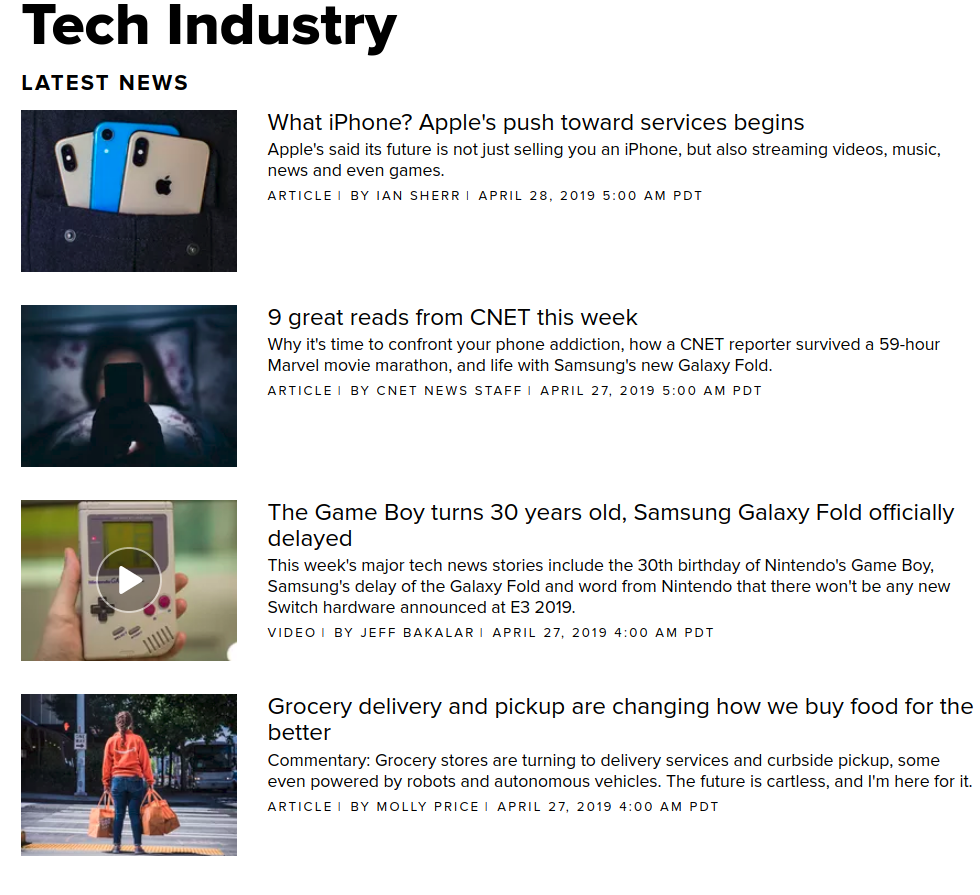
\includegraphics[scale=0.3]{cnet}
	\caption{Hình ảnh trang web được chương trình chọn thu thập dữ liệu}
\end{figure}

Chương trình tự động thu thập bài mới vào mỗi ngày nhờ một crontab lập lịch trên máy chủ linux.
\begin{figure}[h]
	\centering
	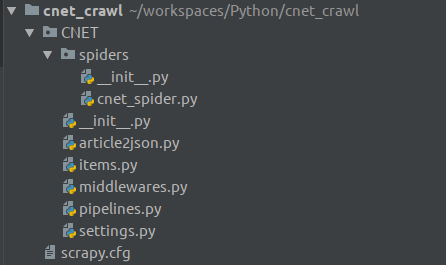
\includegraphics[scale=0.5]{scrapy}
	\caption{Hình ảnh cấu trúc chương trình thu thập dữ liệu}
\end{figure}

\newpage
\newpage
\noindent\textbf{Giao diện ứng dụng hộ trợ đánh giá độ chính xác}

Nhằm để dễ dàng cho những người đánh giá mô hình bài toán trong khóa luận, tôi đã xây dựng một trang web để người dùng thao tác trực tiếp để đánh giá những kết quả đầu ra. 

\begin{figure}[h]
	\centering
	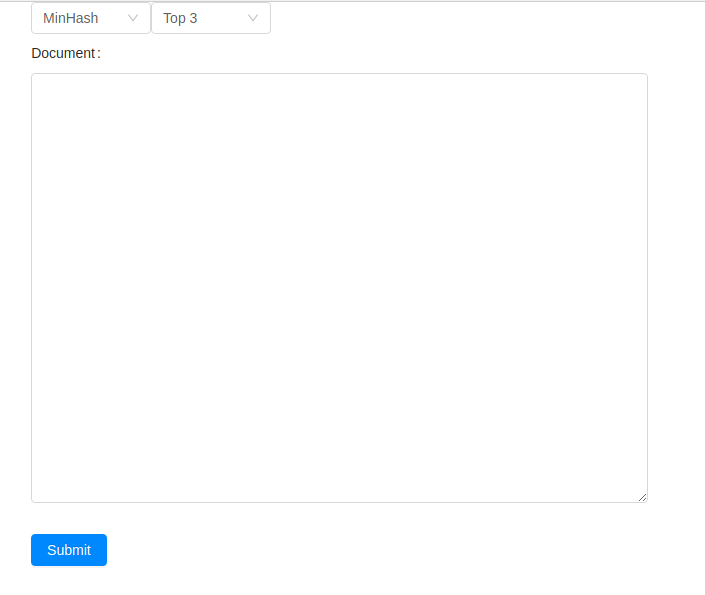
\includegraphics[scale=0.4]{frontend}
	\caption{Hình ảnh giao diện tương tác với người dùng khi chưa có đầu vào}
\end{figure}


\begin{figure}[h]
	\centering
	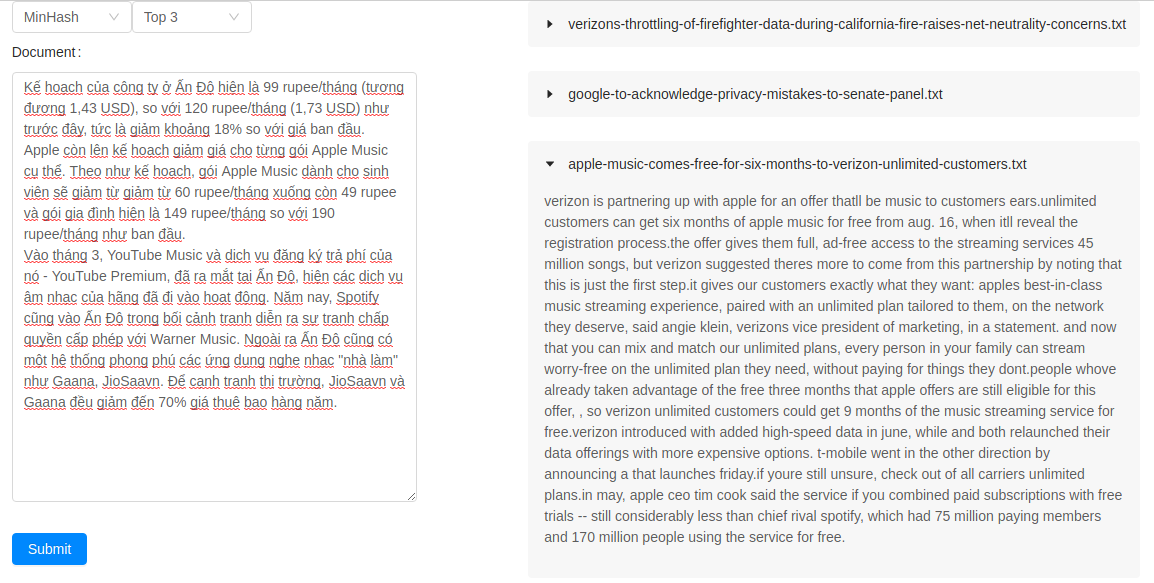
\includegraphics[scale=0.4]{frontend1}
	\caption{Hình ảnh giao diện của chương trình khi người dùng đã tìm kiếm}
\end{figure}


\newpage

\noindent\textbf{Những đánh giá của những người được lựa chọn để kiểm nghiệm mô hình}

\begin{table}[]
	\caption{Nhận xét khi sử dụng chương trình để đánh giá độ chính xác của mô hình đề xuất}
	\begin{tabular}{|l|l|}
	\hline
	\textbf{Họ tên}    & \textbf{Nhận xét}                                                                                                                                                                                                                                                          \\ \hline
	Dương Minh Thu     & \begin{tabular}[c]{@{}l@{}}Kết quả trả về phản hồi khá nhanh, với  phương pháp dùng \\ ma trận những kết quả cần tìm thường được tìm thấy đầu tiên.\end{tabular}                                                                                                           \\ \hline
	Nguyễn Đăng Trường & \begin{tabular}[c]{@{}l@{}}Phản hồi nhanh, những bài tiếng Anh được trả về có chứa \\ những bài không thực sự nên có. Phần lớn là tìm kiếm những\\  bài nói về  công nghệ, chưa tạo ra hệ thống có thể tìm kiếm \\ đa năng các đề tài\end{tabular}                         \\ \hline
	Nguyễn Minh Hiếu   & \begin{tabular}[c]{@{}l@{}}Nhận thấy khi mở rộng tập kết quả trả về sẽ nhận được tỉ lệ\\  kết quả đúng cao hơn, phương pháp này phù hợp với bước \\ tiền xử lý trước khi sử dụng những phương pháp mạnh đòi \\ hỏi công sức tính toán để tìm ra chi tiết hơn.\end{tabular} \\ \hline
	\end{tabular}
\end{table}
\newpage
\section{Kết quả chạy thực nghiệm và đánh giá}

Tại phương pháp thực nghiệm, các từ khóa được lấy ra bằng phương pháp TF. Với cách sử dụng TF-IDF sẽ tạo ra kết quả tốt hơn nhưng lại phải đánh đổi một lượng tính toán cao.

Độ chính xác của ba phương pháp sẽ được đo trên ba phương diện gồm một đoạn văn bản có độ tương đồng nhất, ba đoạn văn bản có độ tương đồng nhất và năm đoạn văn bản có độ tương đồng nhất.

Chương trình dịch được lựa chọn là API của Yandex, API của Google dịch trong nhiều trường hợp sẽ cho kết quả tốt hơn tuy nhiên lại có chi phí khá cao.

Mô hình không gian từ vựng được sử dụng là mô hình \textbf{en core web md}, mô hình được huấn luyện bởi các bài báo, bản tin tiếng Anh do đó sẽ phù hợp với dữ liệu đã được thu thập (được cấp phép bởi MIT).

\textbf{Thực nghiệm độ chính xác của mô hình với việc lấy đại diện cho mỗi văn bản là 15 từ khóa và 10 từ khóa:}

\begin{table}[]
	\centering
	\caption{Bảng đánh giá độ chính xác với 15 từ khóa}
	\begin{tabular}{|l|l|l|l|}
	\hline
												 & Top1 & Top2 & Top3 \\ \hline
	Hàm băm MinHash        & 20\% & 28\% & 32\% \\ \hline
	So sánh cặp ma trận    & 66\% & 74\% & 78\% \\ \hline
	Dịch thuật và uni-gram & 22\% & 32\% & 38\% \\ \hline
	Dịch thuật và 2-gram   & 8\%  & 16\% & 18\% \\ \hline
	\end{tabular}
\end{table}

\begin{table}[]
	\centering
	\caption{Bảng đánh giá độ chính xác với 10 từ khóa}
	\begin{tabular}{|l|l|l|l|}
	\hline
												 & Top1 & Top2 & Top3 \\ \hline
	Hàm băm MinHash        & 20\% & 26\% & 28\% \\ \hline
	So sánh cặp ma trận    & 58\% & 72\% & 76\% \\ \hline
	\end{tabular}
\end{table}

\newpage
Từ bảng trên có thể nhận thấy những phương pháp này đều có những điểm mạnh và điểm yếu riêng: 
\begin{itemize}
	\item Với hướng tiếp cận sử dụng hàm băm MinHash, những kết quả trả về chưa có độ chính xác cao nhưng tỉ lệ chính xác tăng khá nhanh khi tăng số lượng kết quả trả về. Điểm mạnh của phương pháp này là tốc độ truy xuất trên một bộ dữ liệu lớn. Nhận thấy phương pháp này phù hợp với công đoạn lấy tập những văn bản dự tuyển với số lượng lớn trước khi đến công đoạn phân tích chi tiết hơn vì tốc độ truy xuất có thời gian nhanh. 
	\item Với phương pháp ma trận hóa văn bản cho độ chính xác khá cao và tăng dần đế những ngưỡng có thể chấp nhận được tuy nhiên tốc độ truy vấn sẽ tăng rất nhanh khi cơ sở dữ liệu tăng. Phương pháp này có thể phù hợp khi sử dụng sau phương pháp hàm băm vì phương pháp hàm băm đã lọc một lượng lớn những văn bản không cần quan tâm đến, do đó sẽ giảm được những tính toán không cần thiết. 
	\item Phương pháp N-gram có vẻ không thực sự phù hợp với bài toán, phương pháp này sẽ phù hợp hơn khi sử dụng tìm kiếm những văn bản dịch lại toàn bộ không có sửa đổi. Đối với những văn bản trùng lặp về nội dung, ý tưởng, phương pháp này trở nên khá kém.
	\item Phương pháp N-gram càng tăng số lượng gram sẽ trả về kết quả kém đi vì khi đó nó hướng đến việc tìm những đoạn văn bản trùng lặp thông qua một chương trình dịch, cú pháp, cấu trúc câu giữ nguyên khi dịch thuật. Sẽ gặp khó khăn khi bản dịch được thay đổi câu chữ.
	\item Số lượng từ khóa khiến cho độ chính xác của phương pháp hàm băm tăng lên, với phương pháp so sánh cặp ma trận, ý kiên cá nhận nhận thấy độ chính xác sẽ không tăng theo số lượng từ khóa mà sẽ có độ ổn định ở một lượng từ khóa nhất định. 
\end{itemize}

\noindent\textbf{Thảo luận về các kết quả:}

Qua những thực nghiệm trên, tôi nhận thấy với những văn bản có nhiều từ dưới dạng là từ mượn hoặc những từ mang tính xác định một thứ cụ thể và giữ nguyên khi dịch thuật như Google, Facebook\dots khi trở thành từ khóa sẽ đảm bảo toàn vẹn khi qua bước dịch thuật,có chất lượng cao.Tuy nhiên với những từ tên một thương hiệu, hay công ty xuất hiện trong văn bản, mà từ đó lại là một từ có nghĩa khi dịch thuật như Apple ( nếu trở thành từ khóa thì khi dịch thuật để tìm kiếm sẽ trở thành "Quả táo") thì sẽ gây nhầm lẫn cho cả phương pháp sử dụng hàm băm và phương pháp biểu diễn ma trận véc-tơ.



\chapter{Kết luận}
\label{chap:conclusion}

\textbf{Những đóng góp của khóa luận}

Khóa luận này trình bày mô hình tìm kiếm đoạn nội dung tương đồng giữa các văn bản không cùng ngôn ngữ trong đó đầu vào là một văn bản của ngôn ngữ  Việt  và đầu ra là những đoạn văn bản có nội dung tương đồng của ngôn ngữ Anh.

Khóa luận trình bày ý nghĩa của bài toán truy xuất nội dung không cùng ngôn ngữ, từ đó chỉ ra động lực để nghiên cứu, xây dựng khóa luận. Trong đó là những bài toán trích xuất, xây dựng cơ sở dữ liệu từ môi trường web, trích xuất từ khóa của văn bản, truy xuất trong cơ sở dữ liệu lớn.

Khóa luận trình bày và phân tích các hướng để tiếp cận bài toán cho tiếng Việt. Áp dụng các mô hình tìm kiếm nội dung tương đồng của các nghiên cứu đã có cho tiếng Việt cũng như đề xuất phương pháp mới để giải quyết bài toán. Qua đó cho thấy những nghiên cứu đã có cũng có thể đóng góp cho tiếng Việt cũng như phương pháp mới đề xuất cũng có tính triển vọng cao.

Kết quả thực nghiệm phần nào cho thấy sự hoạt động của mô hình đề xuất, là tiền đề để tiếp tục mở rộng bài toán tìm kiếm đoạn nội dung tương đồng cho những văn bản không cùng ngôn ngữ và mở rộng ra là bài toán xác định đạo văn không cùng ngôn ngữ.


\noindent\textbf{Định hướng mở rộng nghiên cứu trong tương lai}

Trong phạm vi của một khóa luận tốt nghiệp, với những hạn chế về kiến thức, thời gian và hạn chế về mặt dữ liệu, mô hình này cần phải được bổ sung nhiều để có thể hoàn thiện hơn nữa.

Đối với mục tiêu cải thiện độ chính xác, tôi xin đề xuất những phương pháp cần được bổ sung và cải thiện như :

Xây dựng mô-đun tách văn bản đầu vào thành các đoạn có cùng nội dung, từ đó có thể xây dựng được tập từ khóa của đoạn văn một cách chính xác hơn

Xây dựng phần dịch máy sử dụng riêng cho mô hình, trong mô hình hiện tại tôi đang đề xuất sử dụng những chương trình dịch đã có sẵn được cung cấp bởi Google và Yandex, tuy nhiên yếu điểm của hai công cụ này là đòi hỏi chi phí khá cao cùng với giới hạn về số lượng từ khi dịch.

Nghiên cứu cải thiện phương pháp trích xuất từ khóa, với phương pháp chỉ sử dụng duy nhất TF sẽ không tạo ra bộ từ khóa hoàn hảo còn khi kết TF-IDF lại tốn một lượng thời gian để tính toán lại toàn bộ những văn bản đã có để lấy giá trị IDF khi xuất hiện một văn bản mới.
\cleardoublepage
\appendix
\section{Phụ lục chương 3}
\begin{figure}[h]
	\centering
	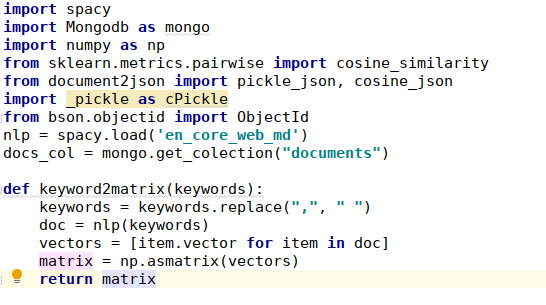
\includegraphics[scale=0.7]{word_embedding}
	\caption{Hàm ánh xạ tập từ khóa sang một ma trận thông qua mô hình không gian từ vựng}
\end{figure}

\begin{figure}[h]
	\centering
	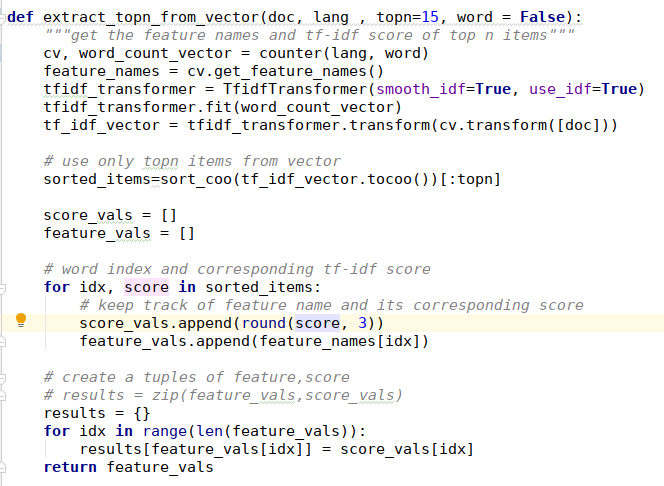
\includegraphics[scale=0.7]{extract_keyword}
	\caption{Hàm trích xuất từ khóa từ văn bản đầu vào sử dụng phương pháp TF-IDF}
\end{figure}

\begin{figure}[h]
	\centering
	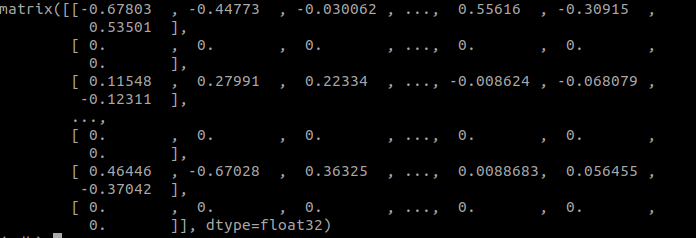
\includegraphics[scale=0.7]{matrix_vector}
	\caption{Ma trận biểu diễn của tập từ khóa sau khi được ánh xạ qua không gian từ}
\end{figure}

\begin{figure}[h]
	\centering
	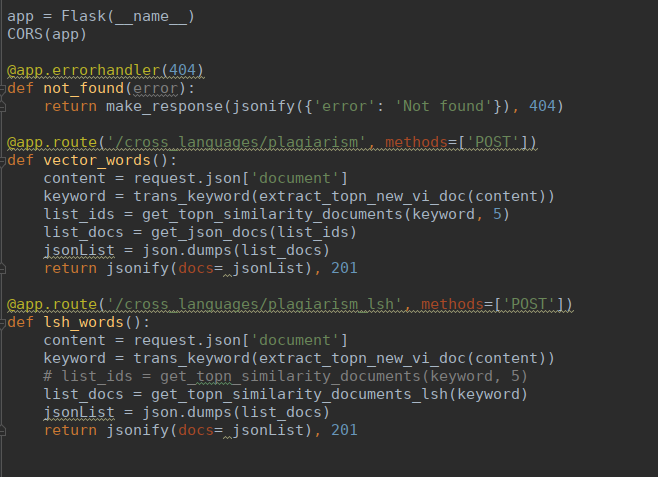
\includegraphics[scale=0.7]{api}
	\caption{Các API từ máy chủ cung cấp cho chương chình tương tác với người dùng}
\end{figure}


\begin{thebibliography}{9}
	\bibitem{cia-ngram} 
	Mcnamee, Paul, and James Mayfield. "Character n-gram tokenization for European language text retrieval." \textit{Information retrieval} 7.1-2 (2004): 73-97.
	
	\bibitem{cia-cross}
	Potthast, Martin, et al. "Cross-language plagiarism detection." \textit{Language Resources and Evaluation} 45.1 (2011): 45-62.
	
	\bibitem{cia-old} 
	Clough, Paul. "Old and new challenges in automatic plagiarism detection." \textit{National Plagiarism Advisory Service, 2003; http://ir. shef. ac. uk/cloughie/index. html.} 2003.
	
	\bibitem{cia-copy} 
	Brin, Sergey, James Davis, and Hector Garcia-Molina. "Copy detection mechanisms for digital documents." \textit{Acm Sigmod Record}. Vol. 24. No. 2. ACM, 1995.
	
	\bibitem{cia-understand} 
	Alzahrani, Salha M., Naomie Salim, and Ajith Abraham. "Understanding plagiarism linguistic patterns, textual features, and detection methods." \textit{IEEE Transactions on Systems, Man, and Cybernetics, Part C (Applications and Reviews)} 42.2 (2012): 133-149.
	
	\bibitem{cia-pairwise}
	Cook, Wade D., and Moshe Kress. "Deriving weights from pairwise comparison ratio matrices: An axiomatic approach." \textit{European Journal of Operational Research} 37.3 (1988): 355-362.
	
	\bibitem{cia-mining}
	Leskovec, Jure, Anand Rajaraman, and Jeffrey David Ullman. \textit{Mining of massive datasets}. Cambridge university press, 2014.

	\bibitem{cia-euclid} 
	Dattorro, J. (2010). \textit{Convex optimization \& Euclidean distance geometry}. Lulu. com.

	\bibitem{cia-word2vec}
	Goldberg, Yoav, and Omer Levy. "word2vec Explained: deriving Mikolov et al.'s negative-sampling word-embedding method." \textit{arXiv preprint arXiv:1402.3722} (2014).

	\bibitem{cia-jaccard}
	Real, Raimundo, and Juan M. Vargas. "The probabilistic basis of Jaccard's index of similarity." \textit{Systematic biology} 45.3 (1996): 380-385.

	\bibitem{cia-tfidf}
	Ramos, Juan. "Using tf-idf to determine word relevance in document queries." \textit{Proceedings of the first instructional conference on machine learning}. Vol. 242. 2003.

	\bibitem{cia-lsh}
	Slaney, Malcolm, and Michael Casey. "Locality-sensitive hashing for finding nearest neighbors [lecture notes]." \textit{IEEE Signal processing magazine} 25.2 (2008): 128-131.

	\bibitem{cia-crawl}
	Shi, Zejian, Minyong Shi, and Weiguo Lin. "The Implementation of Crawling News Page Based on Incremental Web Crawler." \textit{2016 4th Intl Conf on Applied Computing and Information Technology/3rd Intl Conf on Computational Science/Intelligence and Applied Informatics/1st Intl Conf on Big Data, Cloud Computing, Data Science \& Engineering (ACIT-CSII-BCD)}. IEEE, 2016.
\end{thebibliography}

\end{document}
